%!TEX encoding = IsoLatin
\documentclass[a4paper, 11pt,french]{article}
%!TEX encoding = IsoLatin
% ************************
% * fichier de pr�ambule *
% ************************
% ***** extensions *****
\usepackage[latin1]{inputenc}
\usepackage[T1]{fontenc}
\usepackage{lmodern}
\usepackage[english, frenchb]{babel}
\usepackage[pdftex]{graphicx}
\usepackage{subfig}
\usepackage{float}
\usepackage{hyperref}
\usepackage[top=2cm, bottom=2cm, left=2cm, right=2cm]{geometry}
\usepackage[final]{pdfpages} 
\usepackage{amsmath}
\usepackage{amssymb}
\usepackage{mathrsfs}
\usepackage[bottom]{footmisc} 
\usepackage{eurosym}
\usepackage{babelbib}
\usepackage{siunitx}
\geometry{a4paper}
\graphicspath{{media/}}
\renewcommand{\baselinestretch}{1.6}
\selectbiblanguage{french}



% ***** c�sures particuli�res *****
\hyphenation{anti-consti-tu-tionnel-le-ment
atmo-sph�re caou-tchouc cis-alpin trans-action}

% ***** Macros ! *****
\newcommand{\Unit}[1]{\si{#1}}

\begin{document}

\title{Ergom�tre : Rapport de mi-parcours}
\author{Groupe 14}
%\thanks{}
\date{D�cembre 2011}

%%%%%%%%%%%%%%%
%Titre
%%%%%%%%%%%%%%%

\begin{titlepage}
%\maketitle 
\begin{center}
%Universit� Libre de Bruxelles \\


\includegraphics[width=6cm]{ulb.eps}
\hspace{2cm}

\includegraphics[width=6cm]{epb2.eps}
\vspace{6.5cm}
\par{\huge Ergom�tre de Joule-Foucault}
\par  Projet BA\,1 \hspace{0.7cm} 2011-2012
\par
{\large \emph{Rapport final}}
\vspace{2cm}
\par \hrulefill \par
\bsc{Lecomte} Marceau,
\bsc{Marchant} Nikita,


\bsc{Pletschette} Max,
\bsc{Said} Salim,
\bsc{Vekemans} Benoit.


{\emph Groupe 14}
\par \hrulefill \par
\end{center}
\end{titlepage}


%%%%%%%%%%%%%%%
%Abstract
%%%%%%%%%%%%%%%
 ~
\vspace{-8.3cm}
\pagenumbering{roman}
\selectlanguage{english}

\vspace{9cm}
\begin{abstract}
%!TEX encoding = IsoLatin
%!TEX root = ./rapport.tex

\par \textbf{ \og�Ergom�tre de Joule-Foucault�\fg, par Lecomte Marceau, Marchant Nikita, Pletschette Max, Sa�d Salim et Vekemans Benoit, Universit� Libre de Bruxelles, 2011-2012}\\ Nombre de mots~: \num{6478}\\

\par Cette ann�e, le projet BA1 consiste en la construction d'un ergom�tre permettant de chauffer de l'eau  � l'aide des courants de Joule-Foucault. La finalit� est de pouvoir chauffer un volume de \num{10} litres d'eau de \num{3} degr�s en \num{15} minutes, et de d�velopper une puissance de 250 Watt pendant au minimum une minute.

\par Le premier objectif du groupe a �t� de comprendre le principe des courants de Joule-Foucault et de mod�liser leur action sur un conducteur en mouvement.

\par Le dispositif d'entrainement choisi par le groupe est un cyclo-ergom�tre. Celui-ci, d�riv� d'un v�lo conventionnel, est reli� par une cha�ne au caisson contenant le frein magn�tique, partie majeure de l'ergom�tre de Joule-Foucault, constitu� d'une plaque de cuivre et de 8 paires d'aimants dispos�s de part et d'autre de cette plaque.\\ \\ \\


\par\textbf{\og�Joule-Eddy's ergometer\fg, by Marceau Lecomte, Nikita Marchant, Max Pletschette,  Salim Sa�d and Benoit Vekemans, Universit� Libre de Bruxelles, 2011-2012}\\


\par This year's multidisciplinary project of BA1 was to build an ergometer that was able to heat water thanks to the Eddy currents principle. The main goal was to heat a volume of \num{10} liters of water by \num{3} degrees in \num{15} minutes, and to produce a power of \num{250} Watts for at least one minute. The first objective of the group is to understand how Eddy currents work. It has to model it's action on a conducting plate. The chosen machine is a cyclo-ergometer. A regular bicycle was modified for this purpose. The bike is linked to the magnetic brake by an axle and a chain. This system consists of a copper plate rotating between 8 pairs of magnets arranged on either side of the plate.
\end{abstract}
\selectlanguage{french}
\newpage


%%%%%%%%%%%%%%%
%Table des M
%%%%%%%%%%%%%%%
\tableofcontents
\listoffigures
\newpage
\pagenumbering{arabic}


%%%%%%%%%%%%%%%
%Texte !!!
%%%%%%%%%%%%%%%

%Intro
%!TEX encoding = IsoLatin
%!TEX root = ./rapport.tex
\section{Introduction}

Depuis quelques si�cles, la r�volution technologique en marche ne cesse d'amener des nouveaut�s dans beaucoup de domaines, plus vari�s les uns que les autres. Ceci dit, elle soul�ve �galement beaucoup de nouvelles probl�matiques, que les futurs ing�nieurs se doivent de comprendre afin de pouvoir les n�gocier au mieux.\\

Nous vivons actuellement dans un monde ultra technologique, o� beaucoup de t�ches sont automatis�es. La notion m�me d'�nergie est tr�s floue pour beaucoup, tant on dispose d'�lectricit� facilement. Pourtant, il est important de se rendre compte de la quantit� ph�nom�nale d'�nergie qu'on utilise quotidiennement.\\

Ainsi, le projet d'ann�e des �tudiants BA1 en ing�nieur civil propose la r�alisation d'un ergom�tre capable de chauffer de l'eau, en utilisant uniquement les courants de Foucault. Quoi de mieux que de chauffer son eau � la sueur de son front, pour se rendre compte de ce que cela repr�sente~?\\

Au-del� de la probl�matique, mener � bien un tel projet requiert certaines comp�tences, et engendre un r�el apprentissage chez les �tudiants, qui se doivent de passer par diverses �tapes.\\

Ce dossier commencera par mettre en place la th�orie n�cessaire � la compr�hension des courants de Foucault, �l�ment indispensable � la mod�lisation du projet. Cette derni�re sera ensuite d�velopp�e, en expliquant les diff�rents choix auxquels nous avons �t� confront�s. Par la suite, la construction de l'ergom�tre et les exp�rimentations qui ont �t� men�es seront abord�es.\\


\newpage
%Corps
%!TEX encoding = IsoLatin
%!TEX root = ./rapport.tex
\section{Cahier des charges}
\label{sec:cahier}

Extrait de \og Guide du projet BA1 : L'Ergom�tre de Joule-Foucault.\fg~\cite{guide}

\hrulefill \\


Il s'agit de concevoir et fabriquer un \og ergom�tre \fg { }� force de r�sistance magn�tique dont le but est de chauffer de l'eau avec un haut rendement de conversion. Son fonctionnement devra �tre bas� sur l'effet Joule associ� aux courants de Foucault g�n�r�s par le mouvement relatif entre un mat�riau conducteur et le champ magn�tique d'un aimant permanent.\\

L'ergom�tre devra r�pondre aux contraintes suivantes~:

\begin{itemize}
\item La quantit� d'eau � pouvoir chauffer est de 10 litres.
\item La puissance de chauffe pouvant �tre atteinte et maintenue pendant au moins une minute est de 250 Watts.
\item En partant de la temp�rature ambiante, l'eau doit pouvoir �tre chauff�e � un taux de 3�C par quart d'heure.
\item L'ergom�tre doit �tre con�u pour permettre la mesure de la temp�rature en temps r�el.
\item L'ergom�tre doit �tre con�u pour permettre un remplissage et une vidange ais�e de l'eau.
\item La cuve contenant l'eau ne peut pas pr�senter de fuites. Une protection contre les projections d'eau vers l'ext�rieur doit �tre pr�vue aux points d'ouverture s'ils existent.
\item Il faut pr�voir un dispositif simple de mesure des vitesses et des forces que doit exercer l'utilisateur de l'ergom�tre dans diff�rents r�gimes de fonctionnement (si n�cessaire un d�montage partiel rapide pourrait �tre fait pour r�aliser cette mesure).
\item L'ergom�tre doit imp�rativement �tre portable et ses dimensions doivent lui permettre de passer par une porte de dimension standard (il peut �tre d�montable si cela s'av�re n�cessaire au transport).
\item Les pi�ces mobiles en mouvement rapide pr�sentant des dangers de choc ou de pincement doivent faire l'objet de protections ad�quates.
\item La conception de l'ergom�tre devra prendre en compte les contraintes ergonom�triques permettant un usage prolong� sans risque pour l'utilisateur.
\end{itemize}
\newpage
%!TEX encoding = IsoLatin
%!TEX root = ./rapport.tex
\section{Th�orie}
La premi�re �tape du projet consiste � �tablir le cadre th�orique indispensable � la compr�hension des \og courants de Foucault\fg, afin de pouvoir les mod�liser au mieux. Pour ce faire, il est n�cessaire d'�tudier les forces de Lorentz et de Laplace. Ces deux forces forment le frein magn�tique, n�cessaire � l'�l�vation de la temp�rature du conducteur par effet Joule.
Les d�veloppements suivants sont principalement inspir�s des r�f�rences \cite{brown} et \cite{halti}.
\subsection{Force de Laplace}

Soit un conducteur en mouvement plac� dans un champ magn�tique $\vec{B}$, anim� d'une vitesse $\vec{v}$. Une force s'applique sur les charges de ce conducteur (Figure~\ref{fig:lorrentz1}), selon la loi de Lorentz �:
\begin{equation}
	\fbox{$
	\label{eq:lorentz}
	\vec{f_{m}}=q\vec{v}\times\vec{B}
	$}\, ,
\end{equation}
dans laquelle :
 $[\vec{f_{m}}]=\Unit{N}$,
 $[q] =\Unit{C}$,
 $[\vec{v}]=\Unit{m.s^{-1}}$,
$[\vec{B}]=\Unit{T}$.
Ainsi, les charges du conducteur subissant une force $\vec{f_{m}}$ vers le bas, sont anim�es d'une vitesse $\vec{v_{i}}$ (dans le r�f�rentiel du conducteur), amenant les charges positives vers le bas, et par d�faut de charges positives, les charges n�gatives vers le haut (Figure~\ref{fig:lorrentz2}).

\begin{figure}[h]
	\begin{minipage}[t]{6cm}
		\centering
		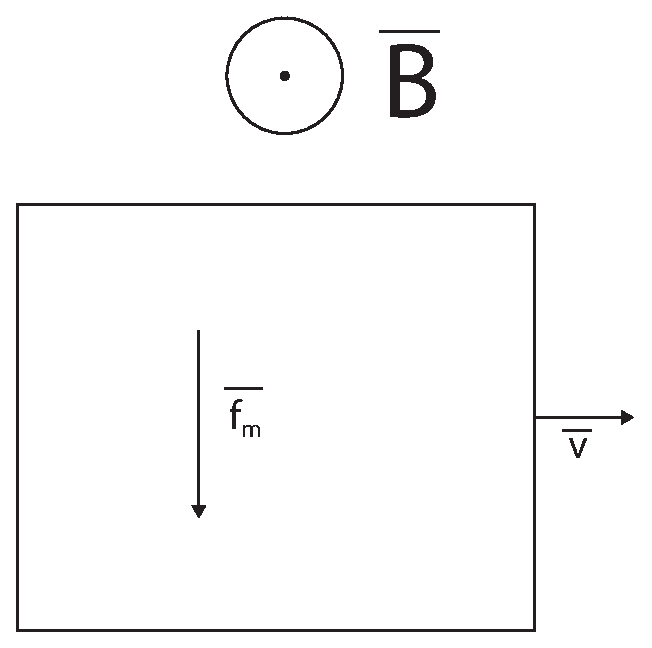
\includegraphics[width=6cm]{schema1.eps}
		\caption{\small \label{fig:lorrentz1}Une Force s'applique sur les charges}
	\end{minipage} \hfill
	\begin{minipage}[t]{6cm}
		\centering
		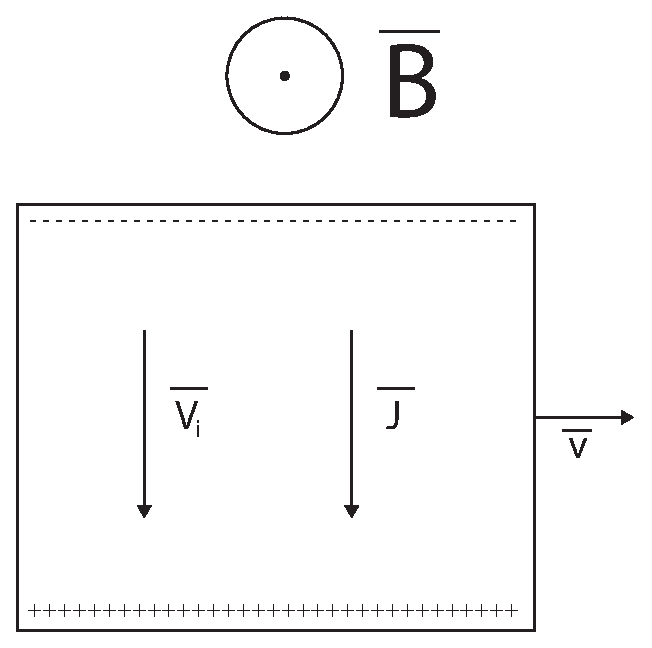
\includegraphics[width=6cm]{schema2.eps}
		\caption{\small \label{fig:lorrentz2}Les Charges descendent}
	\end{minipage}
\end{figure}

On introduit ici la densit� de courant $J$ d�finie par:
\label{sec:densitecourant}
\begin{equation}
	\label{eq:densitecourant}
	J=\frac{I}{S}
\end{equation}
avec $ J=\eta_{e}qv_{i} $ et $[J]=\Unit{A.m.^{-2}}$, $S$ �tant la surface dans laquelle le courant passe ($[S]=\Unit{m^{2}}$).
Les charges anim�es d'une vitesse $\vec{v}_{i}$ et plong�es dans le champ magn�tique $\vec{B}$ subissent � nouveau une force magn�tique $\vec{f}'_{m}$ dans le sens oppos� � la vitesse $\vec{v}$ du conducteur (Figure~\ref{fig:forceopp}).

\begin{figure}[H] %on ouvre l'environnement figure
	\centering
	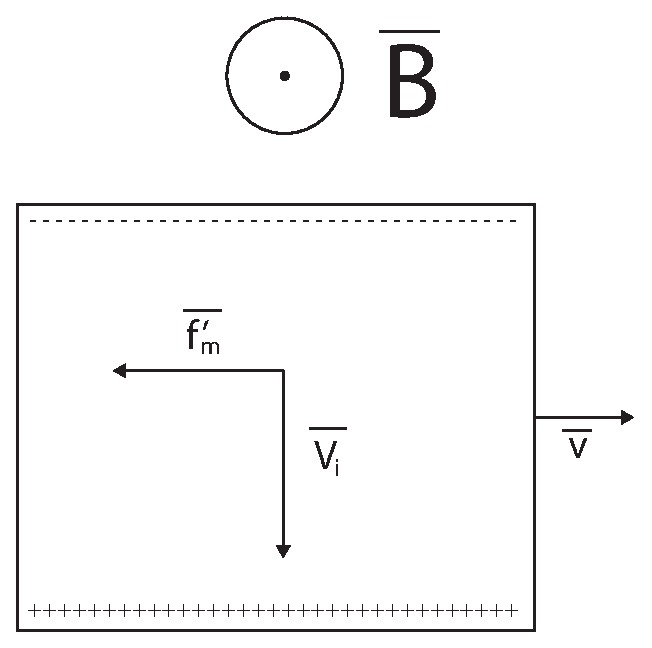
\includegraphics[width=6cm]{schema3.eps} %ou image.png, .jpeg etc.
	\caption{\small Frein magn�tique} %la l�gende
	\label{fig:forceopp} %l'�tiquette pour faire r�f�rence � cette image
\end{figure} %on ferme l'environnement figure
Le conducteur subit ainsi une force $\vec{F}_{M}$ (force de Laplace), dans le m�me sens que $\vec{f}'_{m}$ pour contrer le mouvement initial $\vec{v}$.
La force de Laplace peut �tre vue comme la force de Lorentz au niveau macroscopique.

\subsection{Courants de Foucault}

Malheureusement, cette force de Laplace n'existera pas ind�finiment et donc le frein dispara�tra. En effet, la polarisation du conducteur (s�paration des charges positives et n�gatives) cr�e un champ �lectrique $\vec{E}_{s}$ (Figure~\ref{fig:foucault}), ce dernier provoquant une force $\vec{f}_{E}$ sur les charges. ($ \vec{f_{E}}=q\vec{E_{s}}) $.  Ainsi, quand $ \vec{f_{E}}+\vec{f_{m}}=0 $, les charges ne bougent plus, il n'y a donc plus de force de Laplace.

\begin{figure}[H] %on ouvre l'environnement figure
	\centering
	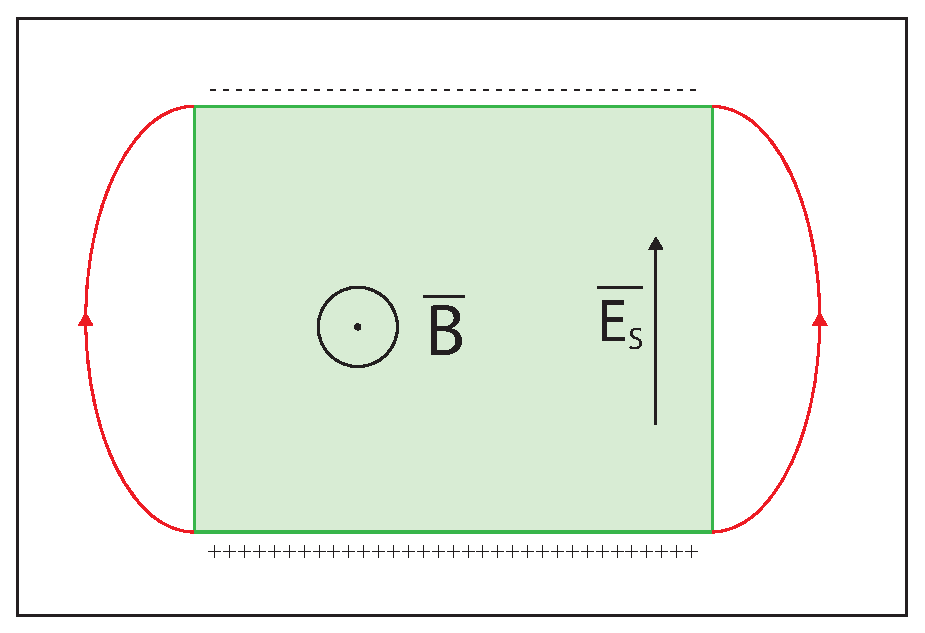
\includegraphics[width=8cm]{schema4.eps} %ou image.png, .jpeg etc.
	\caption{\small Circulation des courants} %la l�gende
	\label{fig:foucault} %l'�tiquette pour faire r�f�rence � cette image
\end{figure} %on ferme l'environnement figure

Il existe cependant une solution~: il suffit de restreindre la zone du conducteur plong�e dans le champ magn�tique, laissant une partie du conducteur hors de ce champ (on admet ici un conducteur beaucoup plus grand que la zone d'entre-fer de l'aimant, en vert sur la Figure~\ref{fig:foucault}).\\

Les charges peuvent donc circuler en dehors de la zone plong�e dans le champ magn�tique $\vec{B}$, sous l'influence du champ �lectrique $\vec{E}_{s}$ (repr�sent� en rouge sur la Figure~\ref{fig:foucault}). Il se forme ainsi une boucle qui ram�ne les charges positives en haut, permettant donc les \og courants de Foucault\fg {} dans le conducteur.

\subsection{Quantification de la force de freinage (frein magn�tique)}
Afin de quantifier la valeur de cette force de Laplace, il est judicieux d'�tablir un parall�le entre la force �lectrique et la force magn�tique. De mani�re g�n�rale, la vitesse des charges $v_{i}$ est proportionnelle � la force �lectrique $f_{E}$ ($[f_{E}]=\Unit{N.C^{-1}}$), qui est elle-m�me proportionnelle au champ �lectrique $E$ ($v_{i}  \varpropto f_{E} \varpropto E_{s} $) Donc~:
\begin{equation}
	\label{eq:mue}
	v_{i}=\mu E_{s},
\end{equation}
O� $\mu$ est une constante qui d�pend du conducteur, appel�e la mobilit� des �lectrons, $[\mu]=\Unit{m^2.V^{-1}.s^{-1}}$. On peut alors faire le rapprochement entre la force �lectrique $f_{E}$ et la force magn�tique $f_{m}$~:
\begin{eqnarray*}
f_{E}&=&qE_{s}, \\
f_{m}&=&qvB, \label{eq:fmagn}
\end{eqnarray*}
($\vec{v}\times\vec{B}=vB$ car $\vec{v}$ et $\vec{B}$ sont perpendiculaires). Nous pouvons donc faire le rapprochement~:
\begin{equation}
	\label{eq:raprochement}
	E_{s}=vB.
\end{equation}
Ce qui donne, dans \eqref{eq:mue}~:
\begin{equation*}
	v_{i}=\mu vB.
\end{equation*}
Rappelons-nous de la densit� de courant $J$ vue au point \ref{sec:densitecourant} dans l'�quation \ref{eq:densitecourant}, et rempla�ons $v_{i}$ par son �quivalent \eqref{eq:mue}~:

\begin{equation*}
	J=\eta_{e}qv_{i}=\eta_{e}q\mu E.
\end{equation*}
Introduisons ici $ \sigma=\eta_{e}q\mu $, la conductivit� �lectrique ($[\sigma]=\Unit{S.m^{-1}}$) que l'on peut retrouver dans des tables~:
\begin{eqnarray*}
J & = & \sigma E, \\
J & = & \sigma vB.
\end{eqnarray*}
Par le m�me rapprochement que \eqref{eq:raprochement}~:
\begin{equation*}
	I=S\sigma vB.
\end{equation*}
Sch�matisons la zone du conducteur plac�e dans l'entre-fer de l'aimant~:�\\

\begin{figure}[H] %on ouvre l'environnement figure
	\centering
	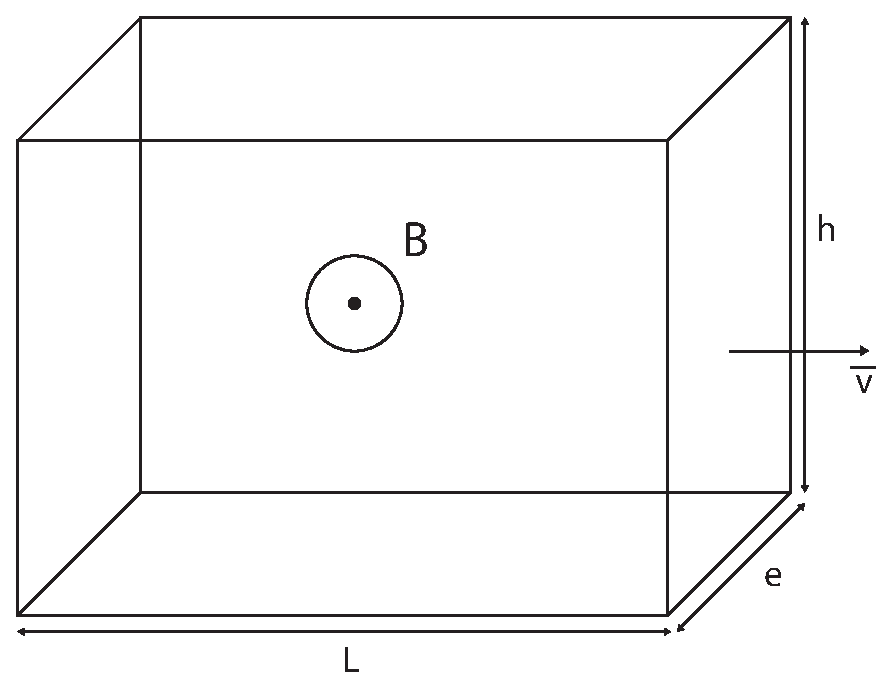
\includegraphics[width=7cm]{schema5.eps} %ou image.png, .jpeg etc.
	\caption{\small Volume dans l'entre-fer} %la l�gende
	\label{volume} %l'�tiquette pour faire r�f�rence � cette image
\end{figure} %on ferme l'environnement figure

D�finissons $\vec{B}$ comme �tant le champ d� � un seul aimant. Comme les aimants sont plac�s face � face, int�ressons-nous � l'intensit� induite par chaque paire d'aimants~:
\begin{equation}
	\label{eq:lhsvb}
	I=2Lh\sigma vB,
\end{equation}
Car $S=Lh$, o� $L$ est la longueur de l'entre-fer, $h$ la hauteur et $I$ l'intensit� du courant ($[I]=\Unit{A}$). Reprenons notre force de Laplace qui vaut, pour chaque paire~:
\begin{equation*}
F_{M}=2IeB, 
\end{equation*}
En rempla�ant $I$ par l'expression d�termin�e ci-dessus \eqref{eq:lhsvb}, on a, pour la force de Laplace~:
\begin{equation*}
F_{M}=4eLh\sigma vB^2,
\end{equation*}
$eLh$ �tant le volume de conducteur plac� dans l'entre-fer ($[eLh]=\Unit{m^3}$). La force totale sera donc~:
\begin{equation}
	\fbox{$
	\label{eq:formulefinale}
	F_{M}=4NeLh\sigma vB^2
	$}\, , 
\end{equation}
$N$ �tant le nombre de paire d'aimants. On arrive enfin � l'expression de la force magn�tique (frein magn�tique) proportionnelle � la vitesse.
\begin{equation}
	\fbox{$
	\label{eq:formulelambda}
	F_{M}=\lambda v
	$}\, ,
\end{equation}
$\lambda$ �tant donc constant pour une m�me configuration des aimants et du conducteur, et valant~:
\begin{equation*}
\label{eq:lambdatheo}
\lambda=4NeLh\sigma B^2.
\end{equation*}
L'�quation \ref{eq:formulefinale} permet de mod�liser au mieux l'ergom�tre. En effet, en contr�lant les diff�rents param�tres de configuration, on peut atteindre la puissance d�sir�e. ($P=F\, v$)\\
L'�quation \ref{eq:formulelambda}, quant � elle, permettra de comparer facilement les donn�es exp�rimentales � la th�orie.

\newpage
%!TEX encoding = IsoLatin
%!TEX root = ./rapport.tex
\section{Choix de l'ergom�tre}
Pour mener � bien ce projet, l'un des points essentiels est le choix de l'ergom�tre.
En effet, la suite des �v�nements s'articule sur cette d�cision.
D�s le d�but, une distinction a �t� faite entre deux types d'ergom�tres: 
les rameurs et les cyclo-ergom�tres.
\subsection{Rameur}
Bien qu'�tant tous les deux capables de remplir le cahier des charges, les cyclo-ergom�tres et les rameurs pr�sentent beaucoup de diff�rences en termes d'utilisation.
Les rameurs mettent tout le corps humain � l'�preuve (y compris les muscles habituellement peu utilis�s)
et une certaine technique doit �tre mise au point par l'utilisateur pour qu'ils puissent �tre utilis�s de mani�re efficace et s�re.\\

Le rameur pr�sente aussi certaines difficult�s sp�cifiques, telles que la mise en place d'un si�ge mobile ou d'un syst�me d'enroulement de la corde.
Pour que le conducteur puisse tourner de fa�on continue, il faudrait le raccorder au reste du m�canisme par une roue libre, ce qui rajoute encore un obstacle.

\subsection{Cyclo-ergom�tres}
Les cyclo-ergom�tres sont en contrepartie plus simples � utiliser. Ils font uniquement appel � des muscles fort entrain�s et ne n�cessitent pas d'adopter une technique d'utilisation particuli�re. La seule partie mobile est la transmission.

Plusieurs types de cyclo-ergom�tres ont �t� �tudi�s~:
\begin{itemize}
\item les v�los \og�assis�\fg, 
\item les v�los \og�couch�s�\fg 
\item les v�los elliptiques.
\end{itemize}
Le dernier type �tant trop difficile � fabriquer et peu puissant, il a �t� �limin� assez rapidement. Les diff�rences entre les deux autres types de v�los sont assez minimes, la principale diff�rence �tant la position de l'utilisateur. L'avantage du v�lo couch� est qu'il sollicite moins le coeur~\cite{erometreassis} qu'un v�lo classique. En effet, l'utilisateur �tant couch�, le muscle cardiaque doit fournir moins d'effort pour remonter le sang des jambes qu'en position assise. Cependant, r�cup�rer un v�lo couch� s'est r�v�l� hors de prix, voire infaisable, et en fabriquer un se serait montr� fort compliqu� ou, dans le meilleur des cas, aurait n�cessit� de lourds travaux de soudure. Un autre avantage du v�lo classique est son syst�me de vitesses d�j� int�gr�, ce qui peut permettre une forte d�multiplication ainsi qu'une souplesse dans celle-ci.
\subsection{Conclusion}

\begin{table}[H]
����\begin{tabular}{| p{4cm} | p{5.2cm} | p{5.3cm} |}
		\hline
��������Ergom�tre����������� & Avantage  & D�savantage \\
		\hline 
��������V�lo elliptique &  Fait travailler bras et jambes &  R�cup�ration impossible \newline Faible puissance\footnote{} \\
		\hline
��������Rameur��������� & Utilise beaucoup de muscles \newline R�cup�re l'�nergie �lastique\footnote{}  & Fatigue trop rapidement\newline R�cup�ration impossible  \newline Technique � apprendre \newline Beaucoup de parties mobiles  \\
		\hline
��������V�lo couch頠�� & Sollicite moins le coeur & R�cup�ration impossible \\
		\hline
��������V�lo assis����� & R�cup�ration possible \newline Mouvement continu \newline Syst�me de vitesses  & Rendement pas maximum\footnotemark[2] \\
		\hline
	\end{tabular}
	\caption{\label{tab:ergo} R�capitulatif des avantages et inconv�nients des diff�rents ergom�tres}
\end{table}


\footnotetext[1]{L'amplitude des p�dales �tant trop petite, une grande force serait n�cessaire pour d�velopper un travail suffisant.}
\footnotetext[2]{Une partie de l'�nergie de compression des muscles sous le poids de l'utilisateur en marchant ou en courant est r�cup�r�e � la d�tente, un peu � la mani�re d'un �lastique. En p�dalant, cette �nergie n'est pas r�cup�r�e.}

Le choix s'est finalement port� sur un v�lo assis. Son ergonomie, son syst�me de vitesses, sa simplicit� d'utilisation et de fabrication l'emportant sur les autres ergom�tres.
\newpage
%!TEX encoding = IsoLatin
%!TEX root = ./rapport.tex
\section{Mod�lisation}
Maintenant que la th�orie est �tablie et que l'ergom�tre est choisi, il est temps de passer � la mod�lisation. Le choix des diff�rentes caract�ristiques techniques de l'appareil se fait sur base de deux objectifs majeurs : le confort d'utilisation et la capacit� � remplir les exigences demand�es � moindre co�t.
%!TEX encoding = IsoLatin
%!TEX root = ./rapport.tex
\subsection{Transmission}
\subsubsection{Calculs des rapports de vitesse}
\label{sec:transm}
Afin de savoir � quelle vitesse le conducteur peut tourner, il faut s'int�resser au rapport de vitesse entre le p�dalage et le conducteur. Pour ce faire, la premi�re �tape est de d�terminer exp�rimentalement (� l'aide d'un fr�quence-m�tre) la fr�quence de p�dalage la plus efficace et confortable. Celle-ci est environ de \SI{1,5} tours par seconde, soit \SI{3\pi}{rad\per\second}. Appelons cette valeur $\omega_{1}$.

\begin{figure}[H] %on ouvre l'environnement figure
	\centering
	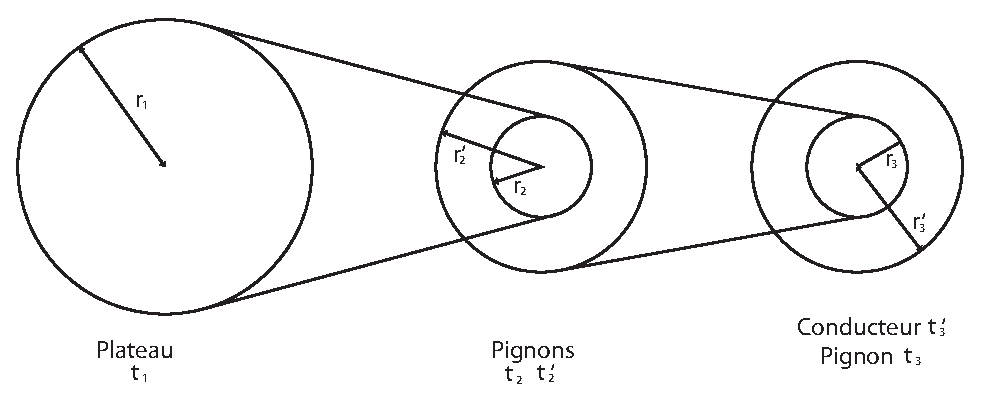
\includegraphics[width=14cm]{transmission.eps} %ou image.png, .jpeg etc.
	\caption{\small Sch�ma de la transmission} %la l�gende
	\label{trans} %l'�tiquette pour faire r�f�rence � cette image
\end{figure} %on ferme l'environnement figure
Pour plus de pr�cision dans les notations, le tableau ci-dessous reprend les diff�rents �l�ments de la transmission ainsi que leurs caract�ristiques.
Comme sur un v�lo classique, le plateau $t_{1}$ est reli� par une cha�ne au pignon $t_{2}$. Une autre cha�ne relie le pignon $t_{2}'$ au pignon $t_{3}$, attach� sur une tige filet�e situ�e � l'arri�re du v�lo, sur laquelle est fix� le conducteur. (Voir Figures \ref{fig:tige} et \ref{fig:chaine})

\begin{table}[H]
\begin{center}
\begin{tabular}{|c|c|c|c|c|}
	\hline nom & type & vitesse angulaire & rayon & vitesse � l'extr�mit� \\
	\hline $t_{1}$ & plateau & $\omega_{1}$ & $r_{1}$ & $v_{1}=\omega_{1}.r_{1}$ \\
	\hline $t_{2}$ & pignon & $\omega_{2}$ & $r_{2}$ & $v_{2}=\omega_{2}.r_{2}$ \\
	\hline $t_{2}'$ & pignon & $\omega_{2}$ & $r_{2}'$ & $v_{2}'=\omega_{2}.r_{2}'$ \\
	\hline $t_{3}$ & pignon & $\omega_{3}$ & $r_{3}$ & $v_{3}=\omega_{3}.r_{3}$ \\
	\hline $t_{3}'$ & conducteur & $\omega_{3}$ & $r_{3}'$ & $v_{3}'=\omega_{3}.r_{3}'$ \\
	\hline
\end{tabular}
\caption{\label{tab:pignons} R�capitulatif des pignons}
\end{center}
\end{table}

La vitesse � l'extr�mit� du plateau ($t_{1}$) est donn�e par~: 
\begin{equation*}
v_{1} = \omega_{1} r_{1}.
\end{equation*}
Or la vitesse � l'extr�mit� de $t_{1}$ est la m�me que celle � l'extr�mit� de $t_{2}$~:
\begin{equation*}
\omega_{1} r_{1} = \omega_{2}r_{2} \Leftrightarrow \omega_{2} = \frac{ \omega_{1}r_{1}}{r_{2}}.
\end{equation*}
Les vitesses angulaires $\omega_{2}$ et $\omega'_{2}$ sont identiques, donc~:
\begin{equation*}
v'_{2} = \omega_{2}  r'_{2} \Leftrightarrow v'_{2} = \frac{ \omega_{1}r_{1}r'_{2}}{r_{2}}.
\end{equation*}
Comme $v_{3}$, la vitesse � l'extr�mit� de $t_{3}$, est la m�me que $v'_{2}$ on a:
\begin{equation*}
	\frac{ \omega_{1} r_{1}.r'_{2}}{r_{2}} =  \omega_{3}r_{3} \Leftrightarrow \omega_{3} =\frac{ \omega_{1} r_{1} r'_{2}}{r_{2} r_{3}}.
\end{equation*}
La vitesse $v'_{3}$ du conducteur $t'_{3}$ vaut donc~:
\begin{equation*} 
v'_{3} = \frac{ \omega_{1} r_{1} r'_{2}}{r_{2} r_{3}} r'_{3}.
\end{equation*}
On a donc finalement la vitesse du conducteur li�e � la vitesse angulaire $\omega_{1}$ et aux diff�rents rayons des pignons.
Faisons appara�tre les rapports $\frac{r_{1}}{r_{3}}$ et $\frac{r_{2}}{r'_{2}}$ dans la relation~:
\begin{equation}
\label{eq:vitessefinale}
v'_{3} = \omega_{1} \left( \frac{r_{1}}{r_{3}} \right)  \left( \frac{r'_{2}}{r_{2}}\right)  r'_{3},
\end{equation}
o� $\frac{r_{1}}{r_{3}}$ et $\frac{r'_{2}}{r_{2}}$ sont �gaux aux rapports des dents sur chacun des pignons et o� $r'_{3}$ est le rayon du conducteur. En utilisant les rapports les plus longs du v�lo, la vitesse du conducteur devient~:
\begin{equation*}
v'_{3} = 3\pi\, \left( \frac{42}{16} \right) \, \left( \frac{30}{14}\right) \, 0,07 = \num{3,7} \Unit{m.s^-1}.
\end{equation*}
\subsubsection{Force appliqu�e sur les p�dales}
La force appliqu�e sur les p�dales n'est autre que~:
$$F = \frac{P}{v},$$
o� $P$ est la puissance ($[P]=\Unit{W}$) et $v$ est la vitesse de p�dalage (vitesse � l'extr�mit� des manivelles, o� $[v]=\Unit{m.s^{-1}}$).
La vitesse angulaire de p�dalage �tant $\omega_{1}=3\, \pi \, \Unit{rad.s^{-1}}$ et la longueur de la manivelle $l=\num{0,17}\Unit{m}$, 
la vitesse $v$ est donc de~:
\begin{equation*}
v = \omega_{1} l = 3\, \pi \, \num{0,17} = \num{1,60} \Unit{m s^{-1}}.
\end{equation*}
La force que l'utilisateur doit appliquer sur les p�dales est alors de~:
\begin{equation*}
\frac{250}{1,60} = \num{156,25} \Unit{N}.
\end{equation*}
Cette valeur obtenue de la force rentre parfaitement dans les plages d�crites par R. Leca \cite{pedale} � propos des capacit�s humaines.


%!TEX encoding = IsoLatin
%!TEX root = ./rapport.tex
\subsection{Frein magn�tique}

\subsubsection{Choix du conducteur}
\label{sec:conduct}
Les deux crit�res principaux dans le choix du conducteur sont sa conductivit� �lectrique et son prix.
Les deux m�taux utilisables sont donc le cuivre et l'aluminium. En effet, ce sont ceux qui ont les plus grandes conductivit�s �lectriques mis � part l'argent et l'or qui sont beaucoup trop chers (voir le tableau~\ref{tab:conducteurs}).\\

Apr�s une recherche dans diff�rents magasins et sites web, il a �t� possible de trouver du cuivre relativement bon march�. Malgr� un rapport conductivit� �lectrique/prix un peu inf�rieur � celui de l'aluminium, la conductivit� sup�rieure (\num{58,0e6} \Unit{S m^{-1}} \cite{conductivite}) du cuivre permet d'utiliser une plaque plus fine et donc de perdre moins de champ magn�tique, cela permettant de faire des �conomies sur l'achat des aimants.
\begin{table}[H]
\begin{center}
\begin{tabular}{|c|c|}
	\hline M�tal & Conductivit� (\Unit{S.m^{-1}}) \\
	\hline Argent & $\num{62,1e6}$ \\
	\hline Cuivre & $\num{58,0e6}$ \\
	\hline Or & $\num{44,2e6}$ \\
	\hline Aluminium & $\num{36,9e6}$ \\
	\hline
\end{tabular}
\caption{\label{tab:conducteurs} Conductivit� �lectrique des mat�riaux les plus int�ressants~\cite{conduct}}
\end{center}
\end{table} 

\subsubsection{Diminution du champ magn�tique en fonction de la distance}

Les aimants ne pouvant pas �tre plac�s directement contre le conducteur, le champ magn�tique � la surface de ce dernier ne correspond pas au champ magn�tique � la surface de l'aimant. Il a donc fallu mod�liser la perte de champ en fonction de la distance. Heureusement, le constructeur fournit une formule permettant de calculer le champ magn�tique le long de l'axe de sym�trie d'un cylindre (ici $z$)~\cite{densit}~:
\begin{equation*}
B = \frac{B_{0}}{2} \left( \frac{D+z}{\sqrt{R^2+(D+z)^2}}-\frac{z}{R^2+z^2} \right),
\end{equation*}
$B_{0}$ �tant le champ magn�tique � la surface de l'aimant et $B$ le champ au point $z$. $[B_{0}]=[B]=\Unit{T}$, le reste des variables sont en m�tres.

Il a �t� d�cid� de placer les aimants � 5\Unit{mm} du conducteur, cette distance �tant suffisamment faible pour ne pas perdre trop d'intensit� de champ magn�tique et suffisamment grande pour ne pas avoir de frottement.

\begin{figure}[H] %on ouvre l'environnement figure
	\centering
	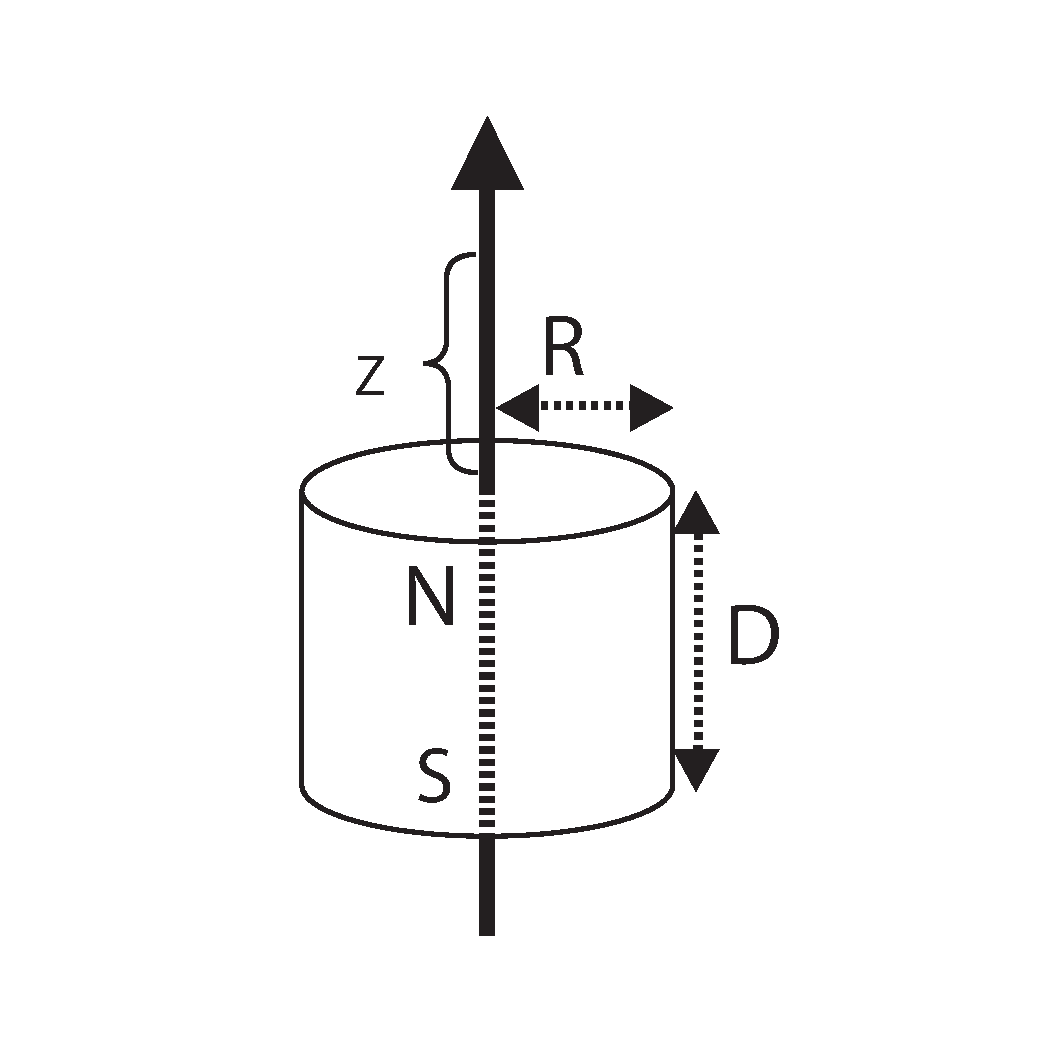
\includegraphics[width=6cm]{champ.eps} %ou image.png, .jpeg etc.
	\caption{\small Sch�ma d'un aimant cylindrique.} %la l�gende
	\label{champ} %l'�tiquette pour faire r�f�rence � cette image
\end{figure} %on ferme l'environnement figure
%Sch�ma des courants de Foucault
\subsubsection{D�termination du nombre d'aimants}
\label{sec:nbaimants}
La force de Laplace $F_{M}$, qui s'oppose au mouvement du conducteur est d�crite par l'�quation \ref{eq:formulefinale} page \pageref{eq:formulefinale}) reprise ici~:
\begin{equation*}
F_{M}=NeLh\sigma v4B^{2},
\end{equation*}
on pose $S = hL$~: surface de l'aimant. La formule devient donc~: 
\begin{equation*}
F_{M}=NeS\sigma v4B^{2}.
\end{equation*}
La puissance d�velopp�e n'�tant rien d'autre que la force multipli�e par la vitesse, la puissance du frein magn�tique peut donc s'�crire comme ceci~:
\begin{equation}P_{M}=NeS\sigma v^{2}4B^{2},
\label{eq:puiss}
\end{equation}
avec $[P_{M}]=\Unit{W}$. Rempla�ons la vitesse par son expression trouv�e au point \ref{sec:transm} dans l'�quation \ref{eq:vitessefinale}~:
\begin{equation*}
P_{M} = \lambda.{v'_{3}}^2,
\end{equation*}
avec~:
\begin{equation*}
\lambda = NeS\sigma4B^{2},
\end{equation*}
et~:
\begin{equation*}
v'_{3} = \omega_{1}.\left( \frac{r_{1}}{r_{3}}\right) .\left( \frac{r'_{2}}{r_{2}}\right) .r'_{3}.
\end{equation*}

Afin de pouvoir calculer le nombre d'aimants, il faut fixer le plus de variables possible. La vitesse du conducteur $v_{3}'$ est connue car les rapports $\frac{r_{1}}{r_{3}}$ et $\frac{r'_{2}}{r_{2}}$ sont connus et que $\omega_{1}$ et $r_{3}'$ sont connus. Comme sp�cifi� dans la section \ref{sec:conduct}, le cuivre est utilis�, ce qui fixe $\sigma = \num{59,6e6}$ \Unit{S m^{-1}}.
Le rayon du conducteur est fix� $r'_{3}$ � $\num{0,07} \Unit{m}$ (arbitrairement).

Le reste des variables d�pendant des aimants, il reste � d�terminer ceux-ci. Trois diff�rents mod�les d'aimants ont alors �t� envisag�s (Voir tableau \ref{ta:aimants}). Pour trouver $N$, il a suffit d'injecter les diff�rentes caract�ristiques des aimants ainsi que les constantes dans l'�quation \ref{eq:puiss} avec $P = \num{250}\Unit{W}$.
\begin{table}[htdp]
\begin{center}
\begin{tabular}{|c|c|c|c|c|}
	\hline R�f�rence & Forme & Diam�tre & Hauteur & R�manence \\
	\hline S-15-08N & disque & 15mm & 8mm & 10,8T \\
	\hline S-25-07N & disque & 25mm & 7mm & 10,8T \\
	\hline S-25-05N & disque & 25mm & 5mm & 10,8T \\
	\hline
\end{tabular}
\caption{\label{ta:aimants} Diff�rents types d'aimants et leurs caract�ristiques \cite{supermagnette}}
\end{center}
\label{defaulttable}
\end{table} 

Pour le premier type d'aimants, cette puissance est atteinte avec 6 paires d'aimants, pour le deuxi�me type d'aimants, 2 paires d'aimants sont n�cessaires pour atteindre les \num{250}\Unit{W} et finalement pour le troisi�me type d'aimants, 3 paires d'aimants sont n�cessaires.

L'utilisation des deuxi�mes et troisi�mes types d'aimants a �t� �cart�e car, en cas de soucis, par exemple si le frein magn�tique est trop faible ou trop fort, l'ajout ou le retrait d'un aimant aurait �t� n�cessaire, ce qui doublerait ou r�duirait de moiti� le champ magn�tique, ce qui n'est �videmment pas une solution.

Le premier type d'aimants a donc �t� choisi. Vu que plus de paires sont n�cessaires � obtenir la puissance demand�e, le nombre d'aimants est plus facilement r�glable en cas de probl�me.

Gr�ce � toutes ces donn�es, il est possible de calculer $\lambda_{th�orique}$ d�fini dans l'�quation~\eqref{eq:lambdatheo}~:
\begin{equation*}
\lambda_{th�orique}=4NeLh\sigma B^2 =  \num{34,7}
\end{equation*}
%
%!TEX encoding = IsoLatin
%!TEX root = ./rapport.tex
\subsection{Appareil de mesure}
\subsubsection{Facteur de proportionnalit� entre puissance et vitesse}
Le but de cet appareil de mesure est de calculer le facteur de proportionnalit� $\lambda$ entre la puissance et la vitesse du conducteur. num�ro de la relation.
En laissant tomber un poids qui est ralenti par la force de Laplace, on observe le poids descendre sur une longueur $L$ dans un temps $\Delta t$. On peut alors d�terminer la vitesse du conducteur car on conna�t le rayon de l'enrouleur $r_{E}$ et le rayon du conducteur $r_{3}'$. 
On admet que sur la distance $L$ le poids n'est pas acc�l�r� et que donc on a une vitesse constante sur cette distance.\\
Reprenons la formule(num�ro de la formule) 
$$\fbox{$ F_{M}=\lambda v$}$$
Dans notre exp�rience on a suppos� la vitesse du poids constant et on peut donc d�duire que la force gravitationnelle sur le poids par la Terre est �gale � la force de Laplace $F_{M}$ \\
$$F_{M} = P$$\\
$P$ �tant la force gravitationnelle du poids en [N]\\
Or $$P = m.g$$\\

$m$ �tant la masse du poids en [kg]\\
La vitesse du poids est la m�me que celle de la bo�te $v_{B}$ car les deux sont reli�s par la m�me corde.\\
On conna�t donc la vitesse angulaire de la tige et donc du conducteur $\omega$\\
$$\omega= \frac{v_{B}}{r_E}$$\\
o� $r_{E}$ est le rayon de la bo�te et donc de l'enrouleur.\\
Et comme le rayon du conducteur est $r_{3}'$ on a la vitesse du conducteur $v$\\

 $$v = \frac{v_{B}r_{3}'}{r_{E}}$$\\
 
 D'ailleurs la vitesse de la bo�te est donn�e par:


$$v_{B} = \frac{L}{\Delta t}$$\\
o� $L$ est la distance parcourue par le poids\\
 $\Delta t$ le temps �coul� pour passer la distance $L$\\

Et donc par(num�roter) on a

$$v = \frac{r_{3}'. L}{\Delta t.r_{E}}$$

Finalement :

$$\lambda = \frac{\Delta t.r_{E}.m.g}{r_{3}'. L}$$

\subsubsection{Calcul de puissance cr�e}
\newpage
%!TEX encoding = IsoLatin
%!TEX root = ./rapport.tex
\section{Construction}

%!TEX encoding = IsoLatin
%!TEX root = ./rapport.tex
\subsection{Ergom�tre}

Apr�s avoir pris la d�cision d'utiliser un cyclo-ergom�tre et apr�s avoir mod�lis� le frein magn�tique, la construction a pu commencer.

L'une des premi�res d�cisions prises concernant la construction fut de ne pas ab�mer le v�lo. Ainsi l'ergom�tre serait adaptable � n'importe quel cycle. 
Un v�lo a donc �t� r�cup�r� et un home-trainer achet� d'occasion\footnote{Le home-trainer a �t� achet� \EUR{50} (voir budget en annexe) et sera revendu en fin d'ann�e}. Gr�ce � ce dispositif, le v�lo est tr�s stable.
\begin{figure}[H] %on ouvre l'environnement figure
	\centering
	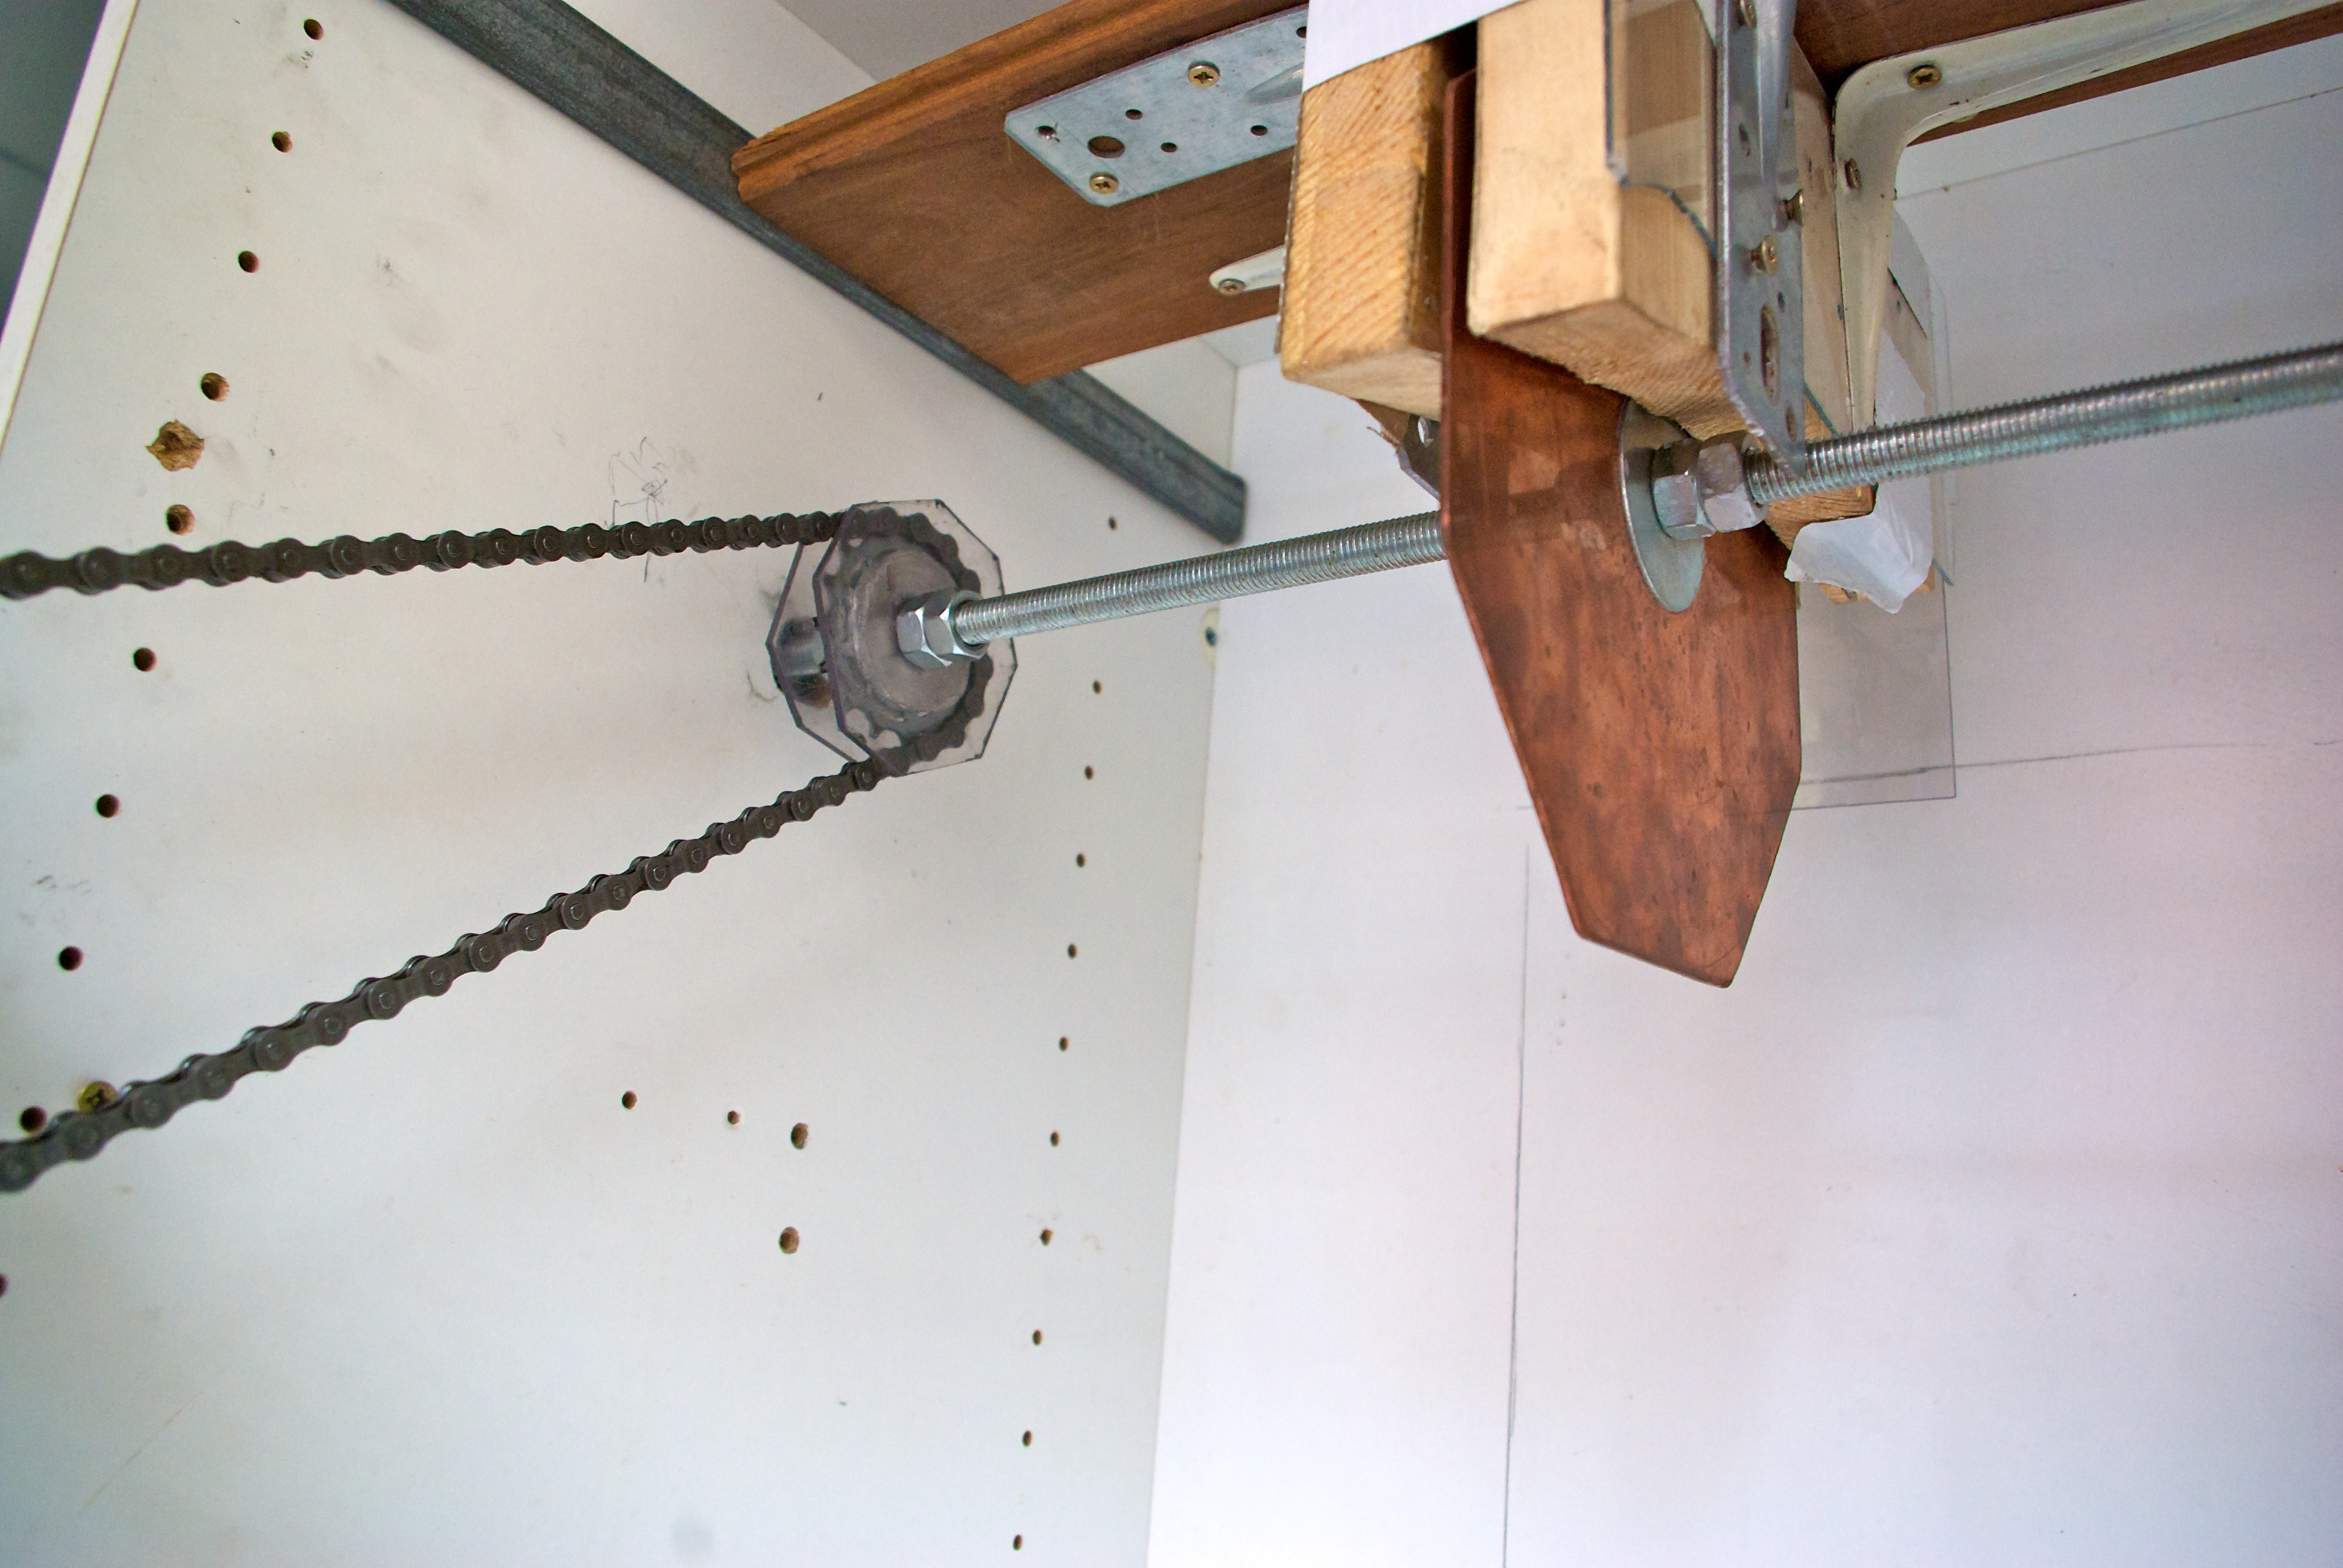
\includegraphics[width=13cm]{photos/tige.jpg} %ou image.png, .jpeg etc.
	\caption{\small Tige filet�e, dernier pignon et conducteur} %la l�gende
	\label{fig:tige} %l'�tiquette pour faire r�f�rence � cette image
\end{figure} %on ferme l'environnement figure
La question s'est alors pos�e sur le dispositif pour faire tourner la plaque du conducteur.
La d�cision a �t� prise de placer le conducteur sur une tige filet�e afin de pouvoir facilement fixer n'importe quelle pi�ce sur l'axe � l'aide d'�crous, gr�ce auxquels un pignon r�cup�r� d'un autre v�lo a �t� fix�.
(Figure~\ref{fig:tige}).
\begin{figure}[H] %on ouvre l'environnement figure
	\centering
	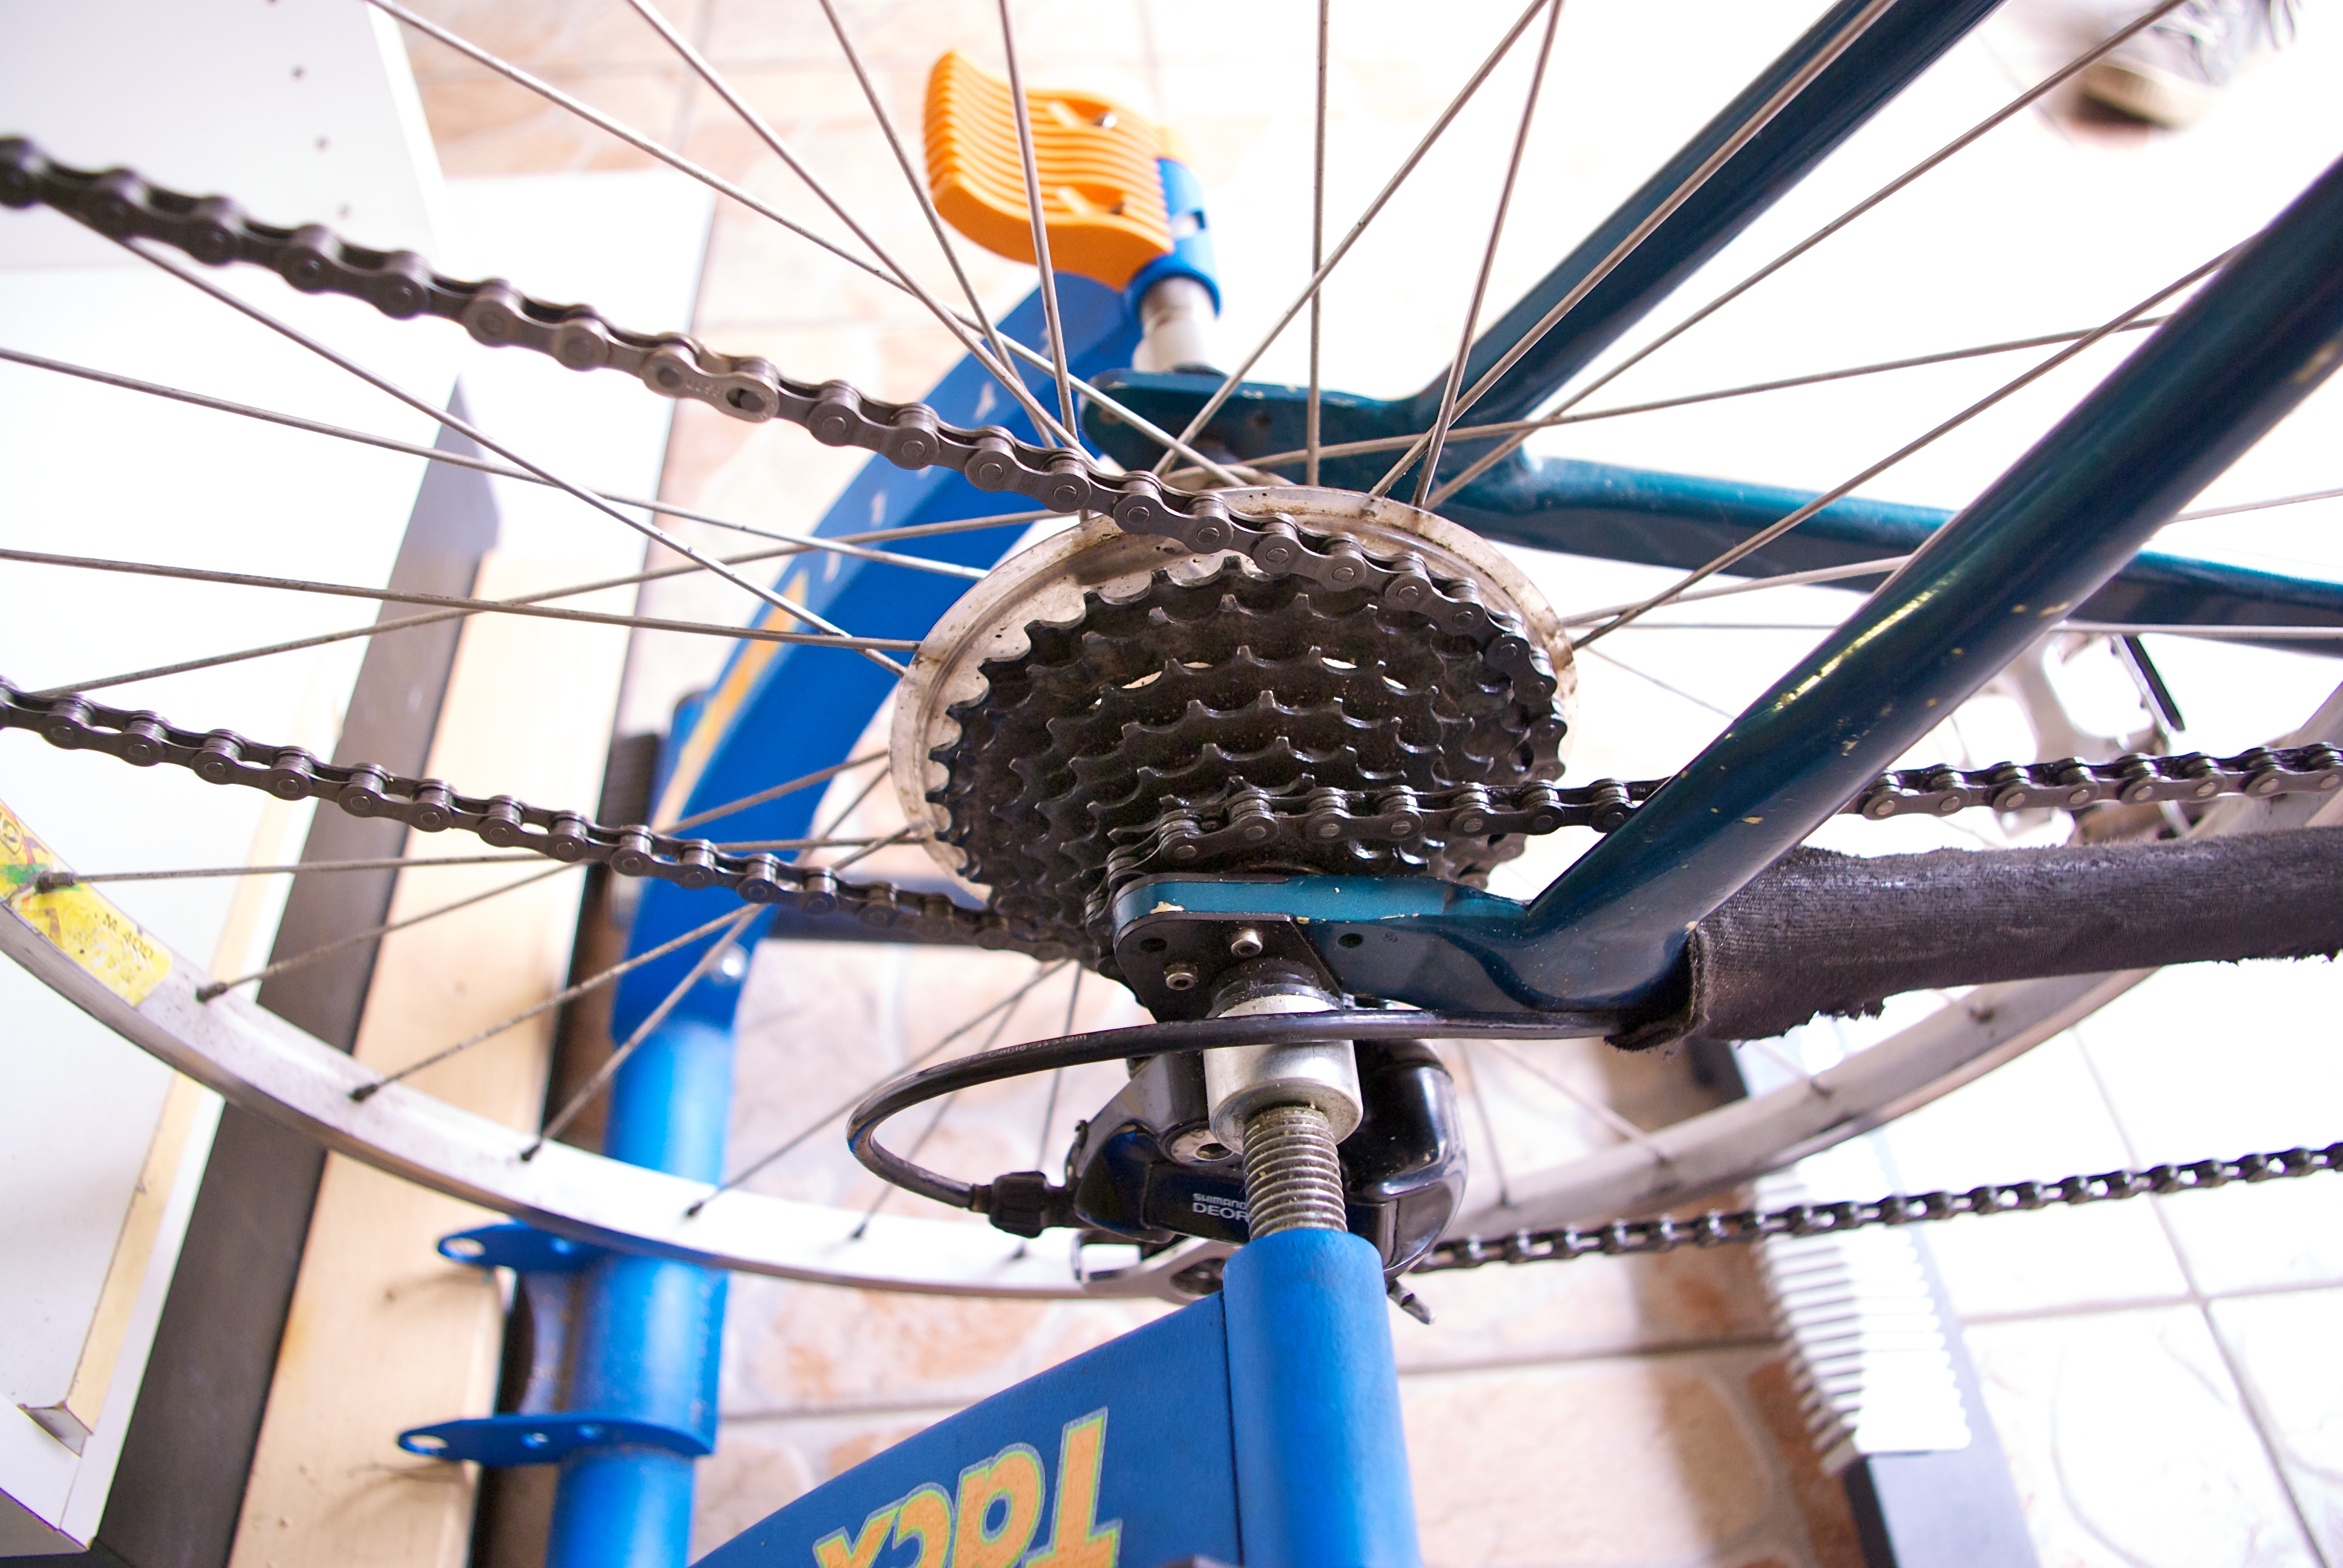
\includegraphics[width=13cm]{photos/chaine.jpg} %ou image.png, .jpeg etc.
	\caption{\small Partie centrale de la transmission} %la l�gende
	\label{fig:chaine} %l'�tiquette pour faire r�f�rence � cette image
\end{figure} %on ferme l'environnement figure


Une deuxi�me cha�ne a ensuite �t� plac�e sur le pignon arri�re du v�lo, reliant celui-ci au pignon de la tige filet�e. Ainsi, en p�dalant, le conducteur est entrain� gr�ce aux deux cha�nes.


%!TEX encoding = IsoLatin
%!TEX root = ./rapport.tex
\subsection{Structure}

Une ancienne armoire a �t� r�cup�r�e, dans laquelle deux trous ont �t� perc�s afin d'y placer des roulements � billes et l'axe du conducteur.

\begin{figure}[H] %on ouvre l'environnement figure
	\centering
	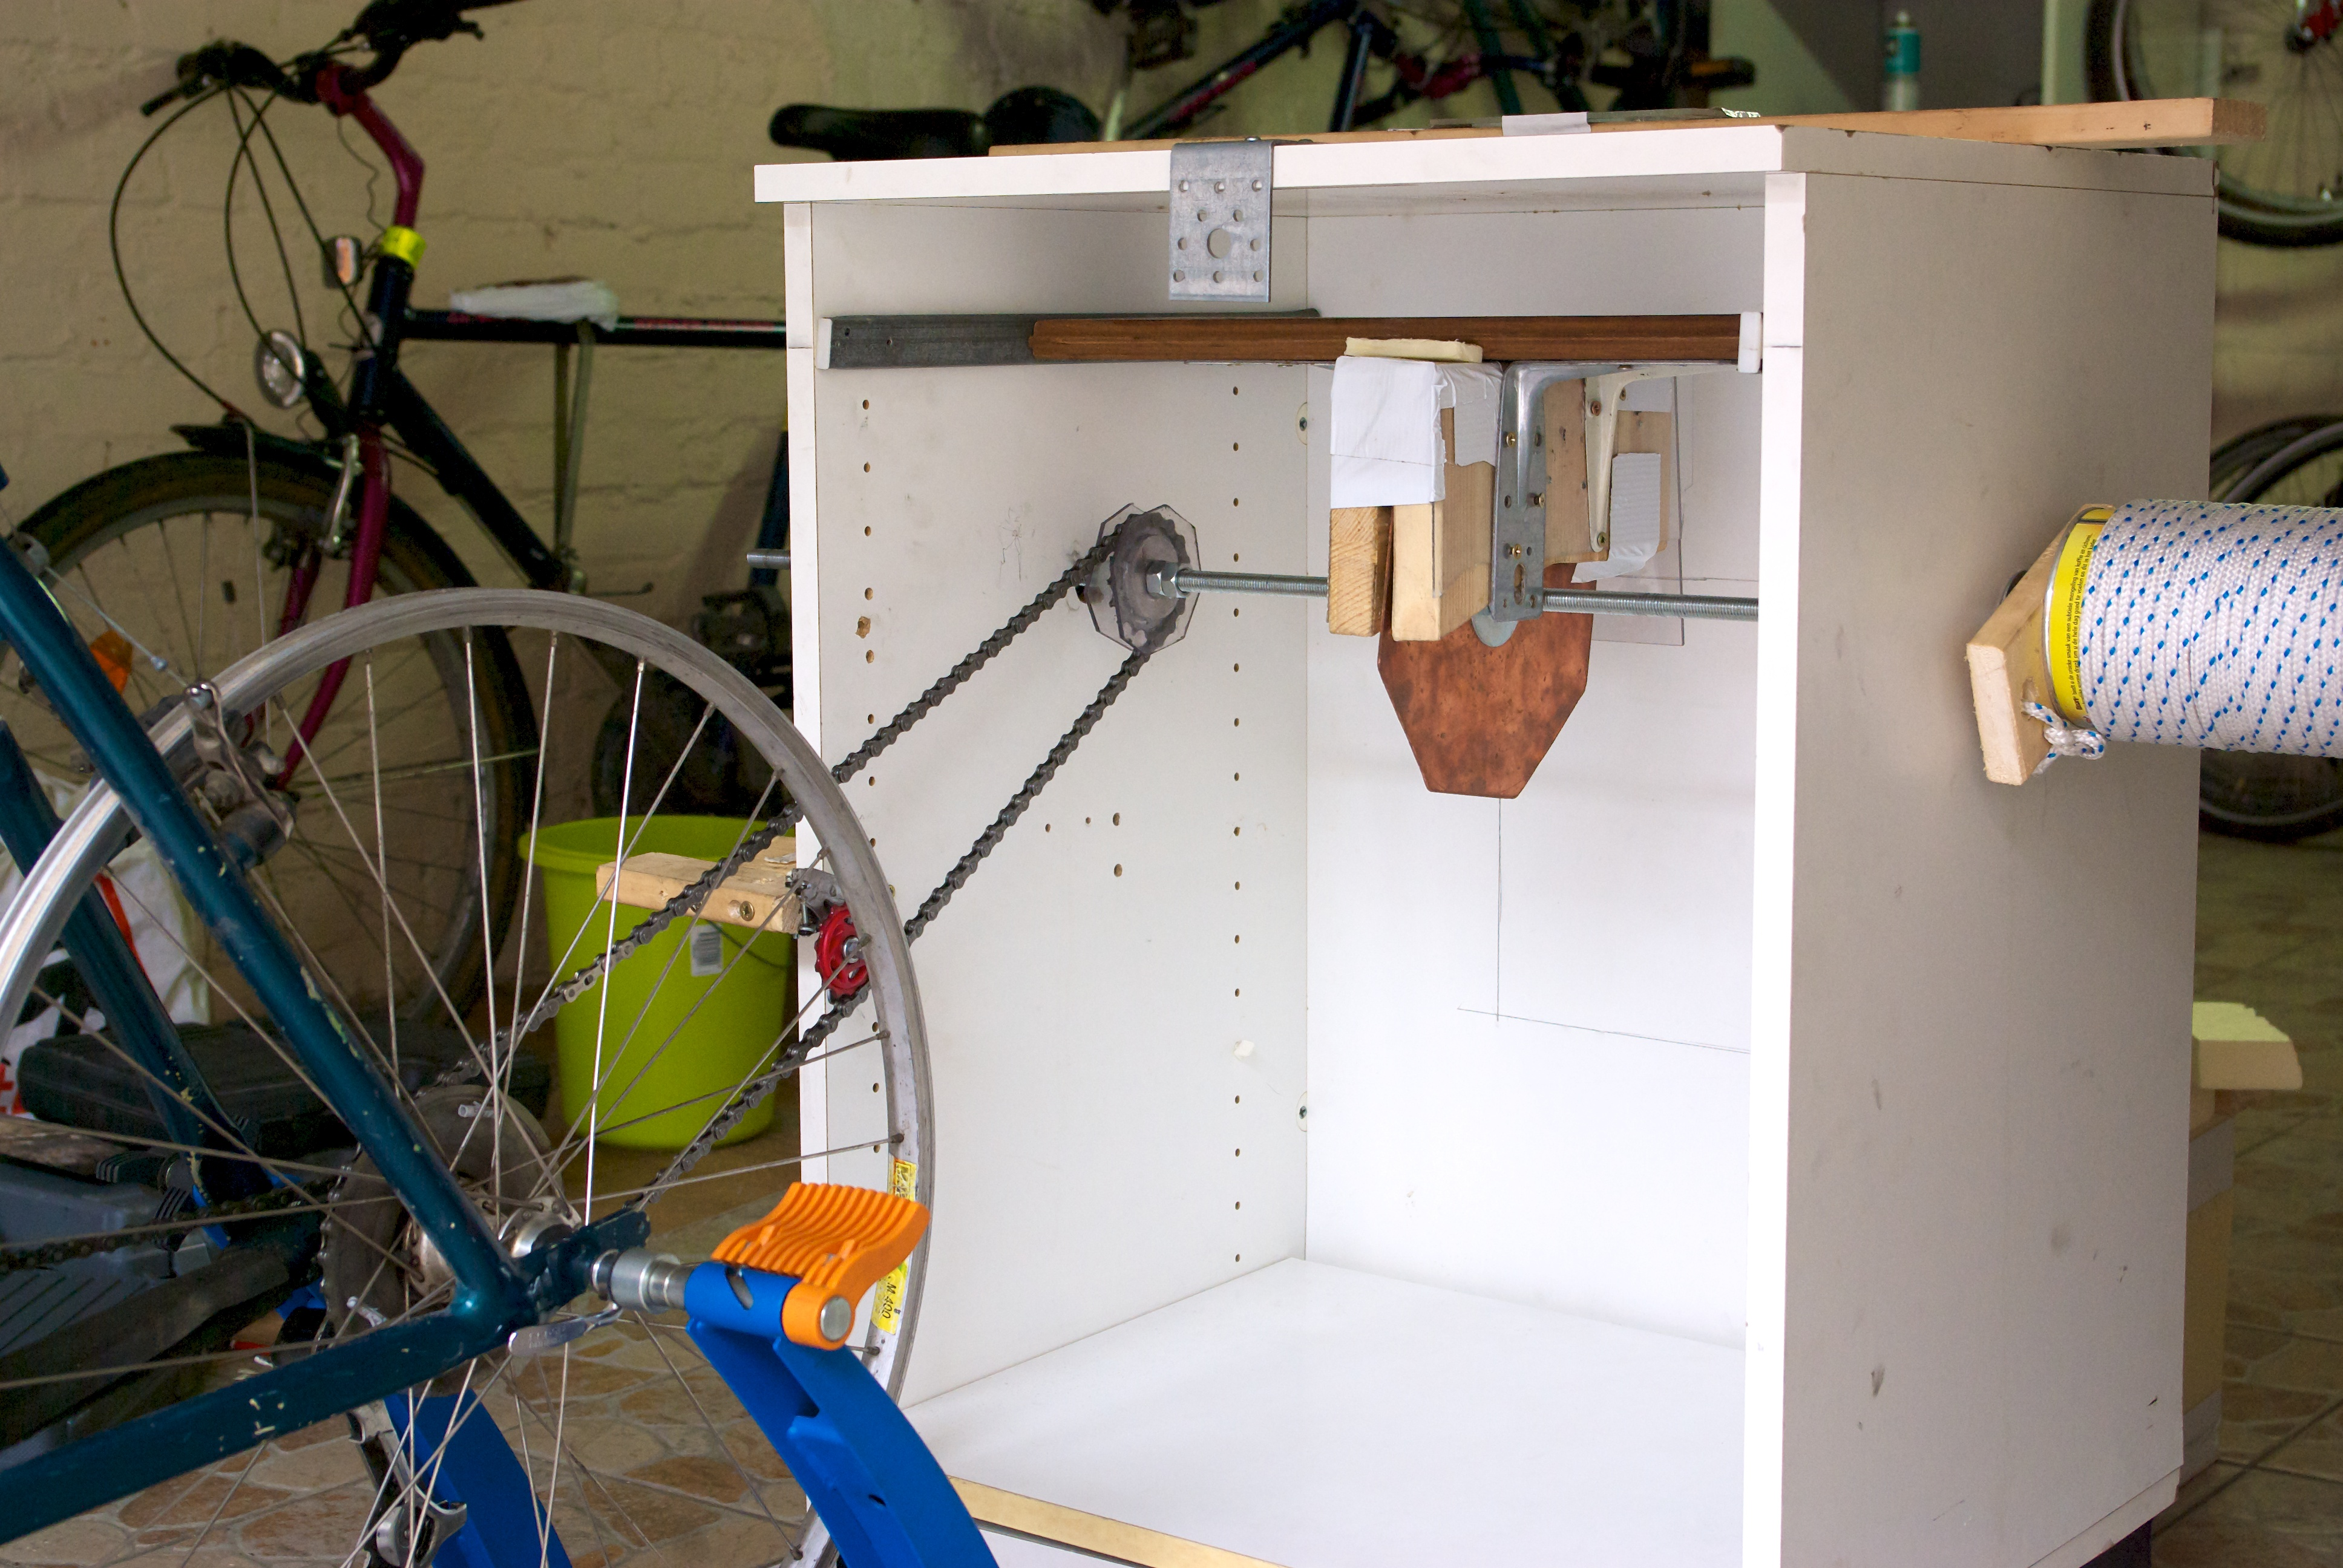
\includegraphics[width=13cm]{photos/construction.jpg} %ou image.png, .jpeg etc.
	\caption{\small Photo de l'ergom�tre} %la l�gende
	\label{fig:ergo} %l'�tiquette pour faire r�f�rence � cette image
\end{figure} %on ferme l'environnement figure

\subsection{Cuve}

La cuve est un �l�ment important de l'ergom�tre. C'est elle qui va contenir les 10 litres d'eau � chauffer. Il est donc n�cessaire qu'elle soit �tanche et isol�e.

Premi�rement, il a fallu choisir un mat�riau. Le choix s'est port� sur du polystyr�ne extrud�, mat�riau usuellement utilis� dans l'isolation de b�timents. Sa solidit� permettant de construire enti�rement la cuve dans ce mat�riau, et sa conductivit� thermique �tant tr�s faible, celui-ci est un mat�riau id�al.

La cuve a �t� assembl�e avec du silicone. L'int�rieur de la cuve a ensuite �t� recouvert d'une couche de mastic �tanche, afin de s'assurer que l'eau ne coulerait pas en dehors de la bo�te.

Pour diminuer les pertes thermiques, un couvercle a �videmment �t� ajout�. Celui-ci a �t� r�alis� en deux parties de fa�on � pouvoir le mettre et l'enlever rapidement et sans encombres. Une encoche est aussi pr�sente pour pouvoir laisser passer le conducteur et l'axe.

\begin{figure}[H] %on ouvre l'environnement figure
	\centering
	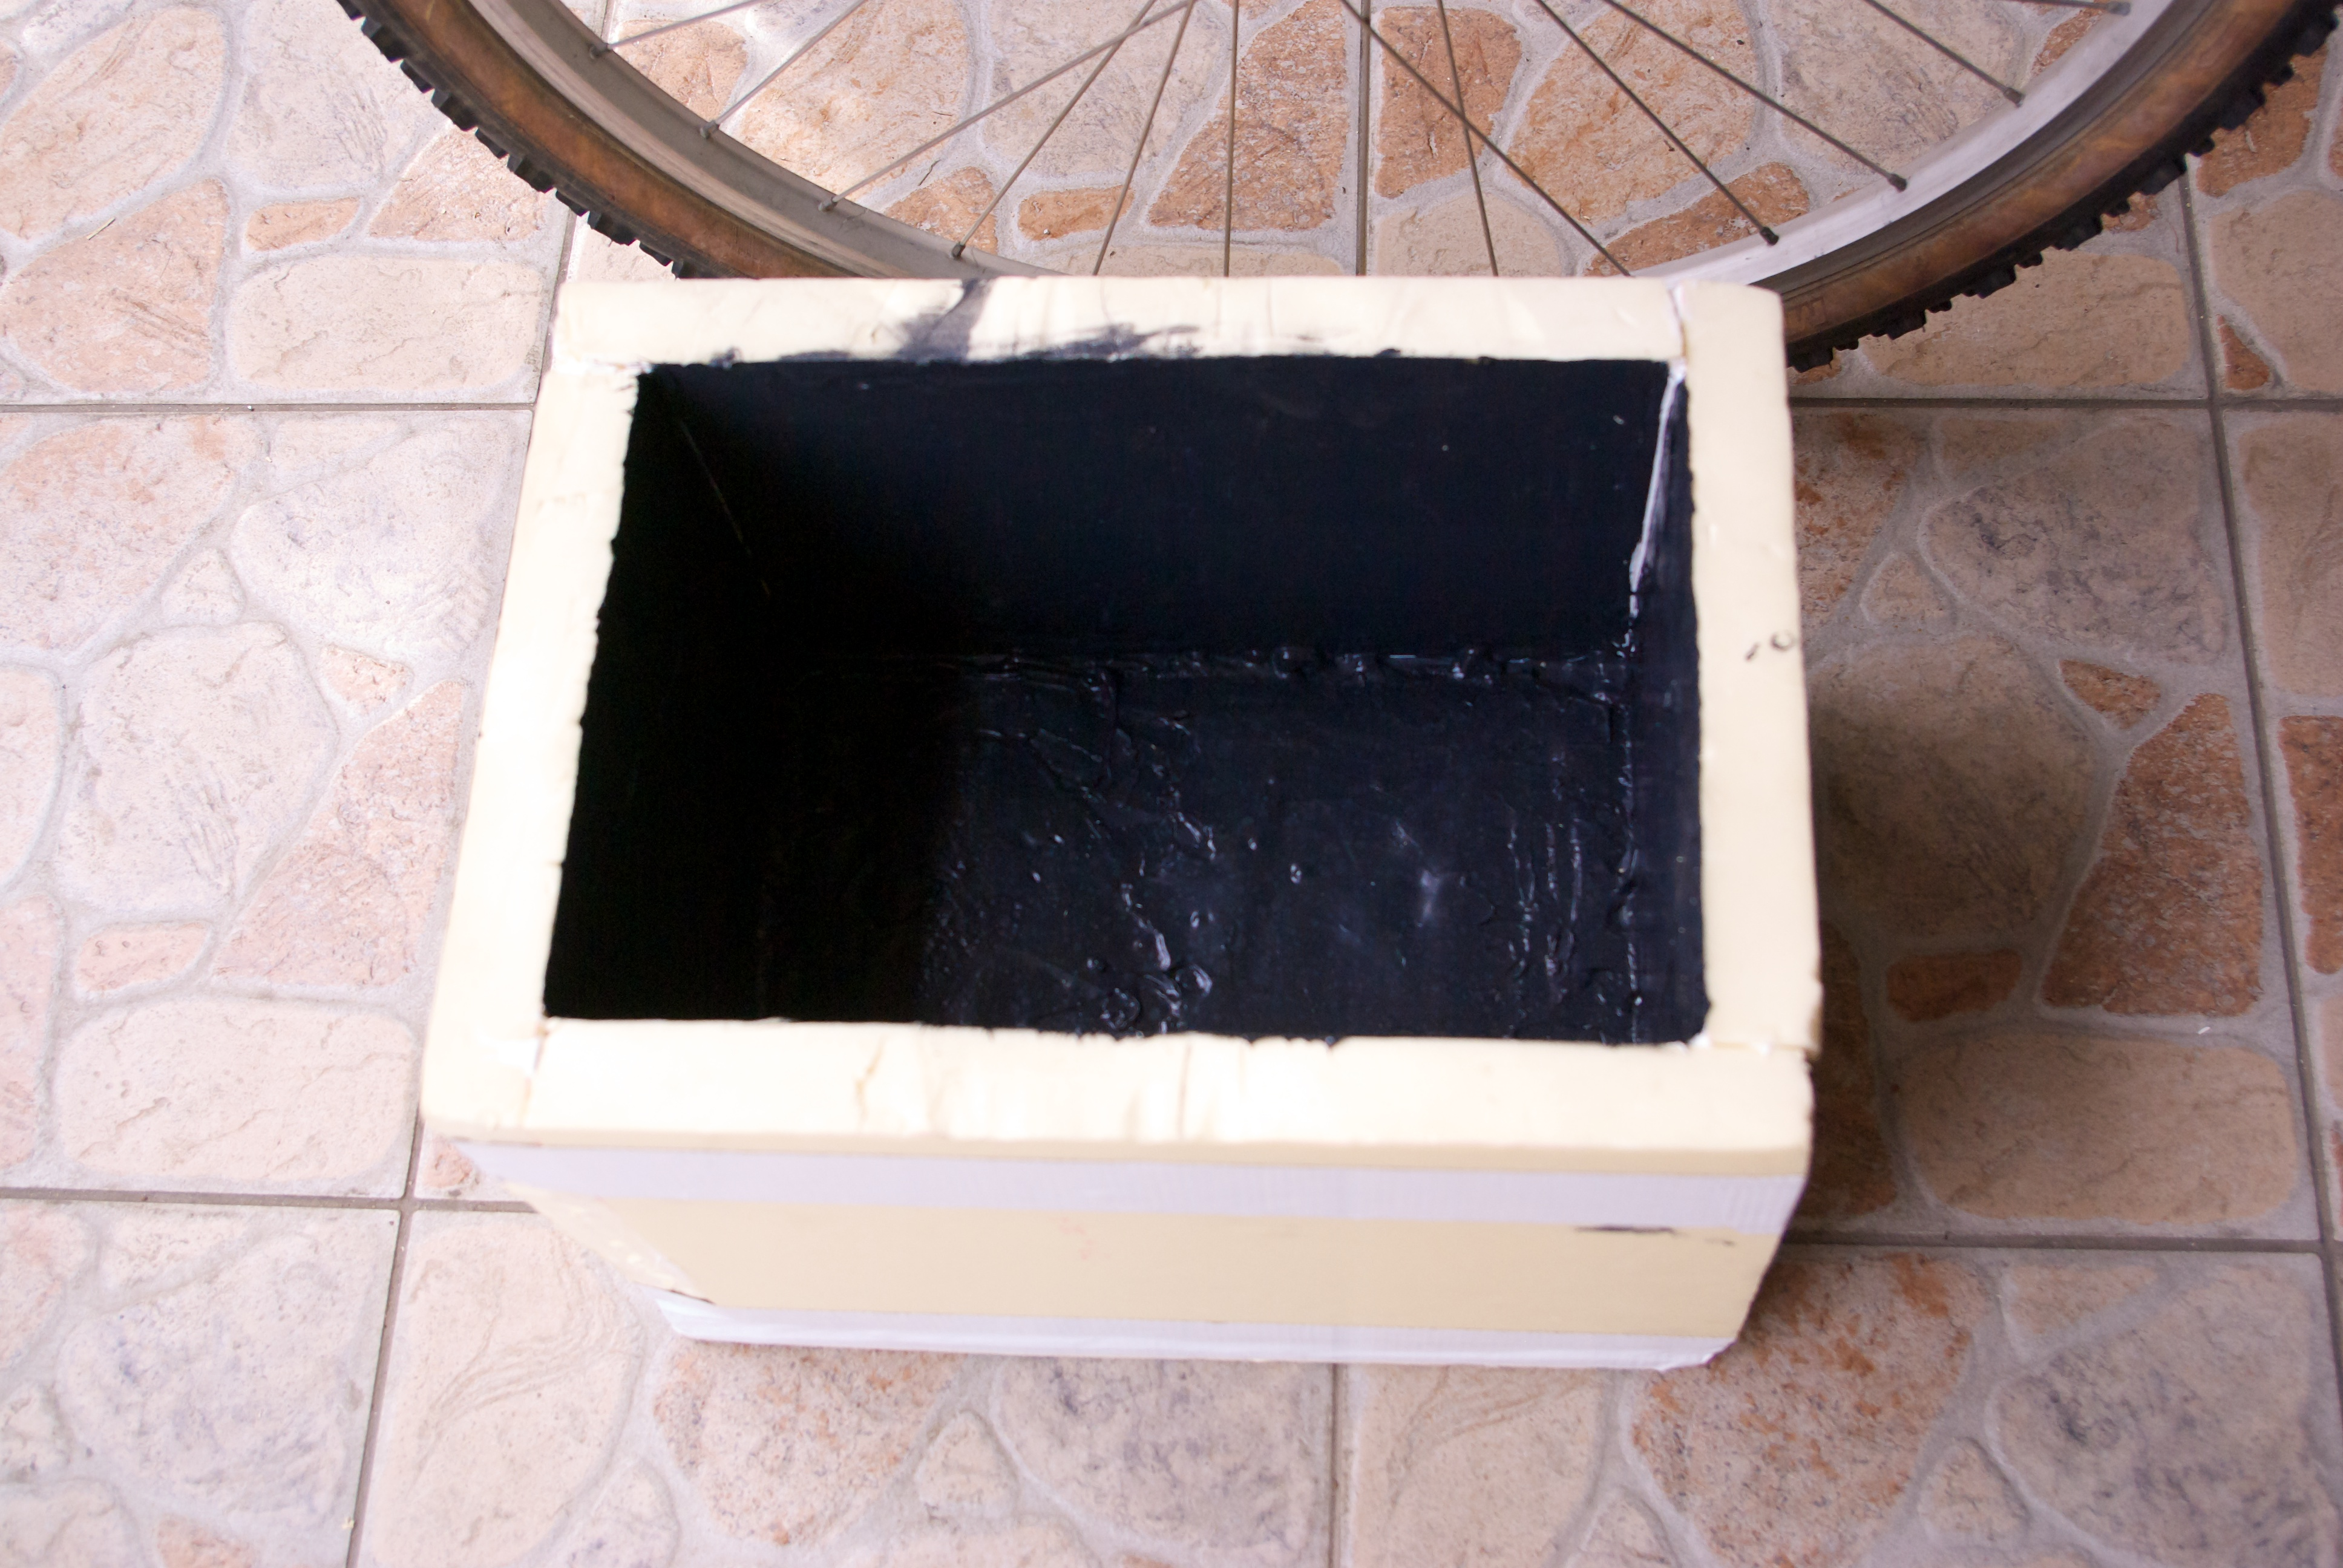
\includegraphics[width=15cm]{photos/cuve.jpg} %ou image.png, .jpeg etc.
	\caption{\small Photo de la cuve} %la l�gende
	\label{fig:cuve} %l'�tiquette pour faire r�f�rence � cette image
\end{figure} %on ferme l'environnement figure

%!TEX encoding = IsoLatin
%!TEX root = ./rapport.tex


%\subsection{Fixation des aimants}

\subsection{Fixation des aimants}

Pour obtenir la vitesse lin�aire du conducteur la plus grande possible, les aimants doivent �tre plac�s le plus loin possible de l'axe de rotation du disque. (en restant n�anmoins dans la zone de conducteur, le but �tant d'obtenir des courants de Foucault). Ceux-ci sont donc plac�s le long d'un arc de cercle de 9 \Unit{cm} centr� sur l'axe du conducteur (voir Figure \ref{fig:dispo}).

Les aimants sont plac�s c�te � c�te avec une polarit� � chaque fois invers�e. Gr�ce � cette technique les courants de Foucault s'intensifient. En effet, � chaque entre-fer d'un aimant se cr�e un champ �lectrostatique et comme les champs magn�tiques sont � chaque fois invers�s, les champs �lectrostatiques de chaque entre-fer sont en alternance � cause de la loi de Lorentz. Ceci donc permet aux �lectrons de compenser le d�faut d'�lectrons de chaque c�t�. Il y a donc deux fois la possibilit� de courants de Foucault~: d'une extr�mit� de l'entre-fer � l'autre et entre deux entre-fers.

\begin{figure}[H] %on ouvre l'environnement figure
	\centering
	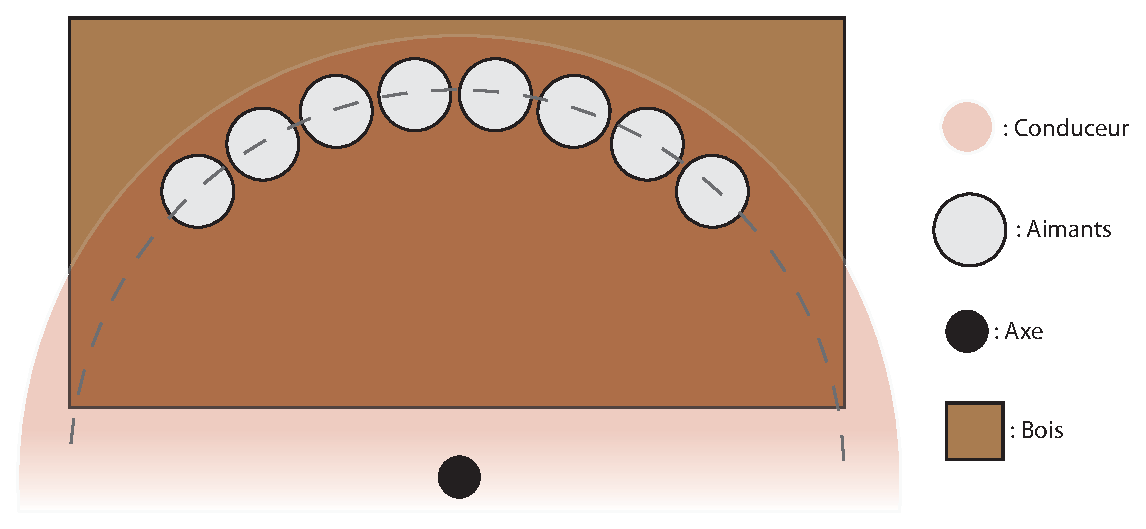
\includegraphics[width=15cm]{dispo_aimants.eps} %ou image.png, .jpeg etc.
	\caption{\small Disposition des aimants} %la l�gende
	\label{fig:dispo} %l'�tiquette pour faire r�f�rence � cette image
\end{figure} %on ferme l'environnement figure


%La fixation des aimants est, l'air de rien, une t�che difficile � r�aliser correctement !
%Les aimants s'attirant fortement, il est difficile de les faire tenir en place afin de les coller.\\

%Afin de les garder � la bonne distance, et surtout pour qu'ils ne bougent pas en permanence, un module s'imposait.
%Voici ce � quoi nous sommes arriv�s :

%\begin{figure}[H] %on ouvre l'environnement figure
%	\centering
%	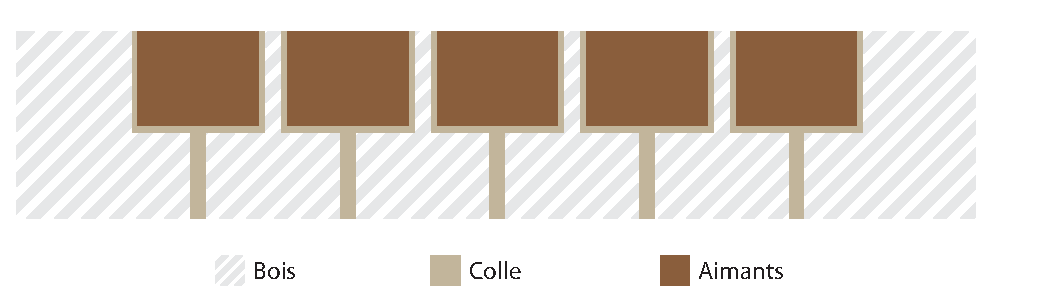
\includegraphics[width=16cm]{aimants.eps} %ou image.png, .jpeg etc.
%	\caption{\small Coupe du module de fixation des aimants} %la l�gende
%	\label{fig:aimants} %l'�tiquette pour faire r�f�rence � cette image
%\end{figure} %on ferme l'environnement figure

%Ainsi, les aimants sont cloisonn�s dans des logettes creus�es dans le bois.
%La colle n'a plus qu'� �tre vers�e, autant par le haut que par le bas !\\
%En effet, dans un soucis de facilit� d'insertion de la colle, nous avons fait des trous de l'autre c�t� de la plaque en bois.\\

%Malheureusement, nous avons fix� nos aimants avec un mastique qui n'a pas tenu la route. En urgence, il a fallu trouver un moyen de pr�senter quelque chose qui %fonctionne pour la validation du pr�-prototype.\\

%Pour ce faire, nous avons r�cup�r� une plaque de Plexiglas d' 1mm d'�paisseur pour maintenir les aimants en place.
%La prochaine �tape est de changer de colle et recommencer avec un nouveau morceau de bois, trou� de la m�me mani�re.





\newpage
%!TEX encoding = IsoLatin
%!TEX root = ./rapport.tex
\section{Exp�rimentations, pertes et rendements}
%!TEX encoding = IsoLatin
%!TEX root = ./rapport.tex
\subsection{Mesures}
Ayant trouv� le lambda th�orique (section \ref{sec:nbaimants}), il faut maintenant trouver le lambda exp�rimental afin de calculer les rendements et de v�rifier que nos pertes ne sont pas trop importantes.
Lambda est d�fini comme liant la puissance au carr� de la vitesse au bord du disque de cuivre. (Voir �quation \ref{eq:formulelambda})
\begin{equation*}
P=\lambda v_{3}'^2
\end{equation*}
Afin de d�terminer $\lambda$, il faut passer par la fabrication d'un appareil de mesure permettant de d�velopper une certaine puissance. Il ne reste donc plus qu'a mesurer la vitesse du conducteur pour d�terminer~$\lambda$.

\subsubsection{Dispositif de mesure}
\label{sec:mesure}
Afin de d�velopper une puissance mesurable, il suffit de laisser tomber des masses dans le champ gravitationnel, pendues � une corde enroul�e autour d'un cylindre centr� sur l'axe sur lequel se trouve le conducteur. L'axe �tant � moins d'un m�tre du sol, il a �t� n�cessaire d'utiliser un poteau d'environ 2 m�tres de haut afin de faire passer la corde par une poulie fix�e au sommet, et ainsi allonger le temps de chute des poids.
Ainsi, en consid�rant que la vitesse de chute est constante (en ne comptant donc pas les premiers instant de chute), la puissance d�velopp�e par la masse n'est autre que~:
\begin{equation*}
P=m_{poids}\,g\,v_{poids}
\end{equation*}

\begin{figure}[h]
	\begin{minipage}[t]{6cm}
		\centering
		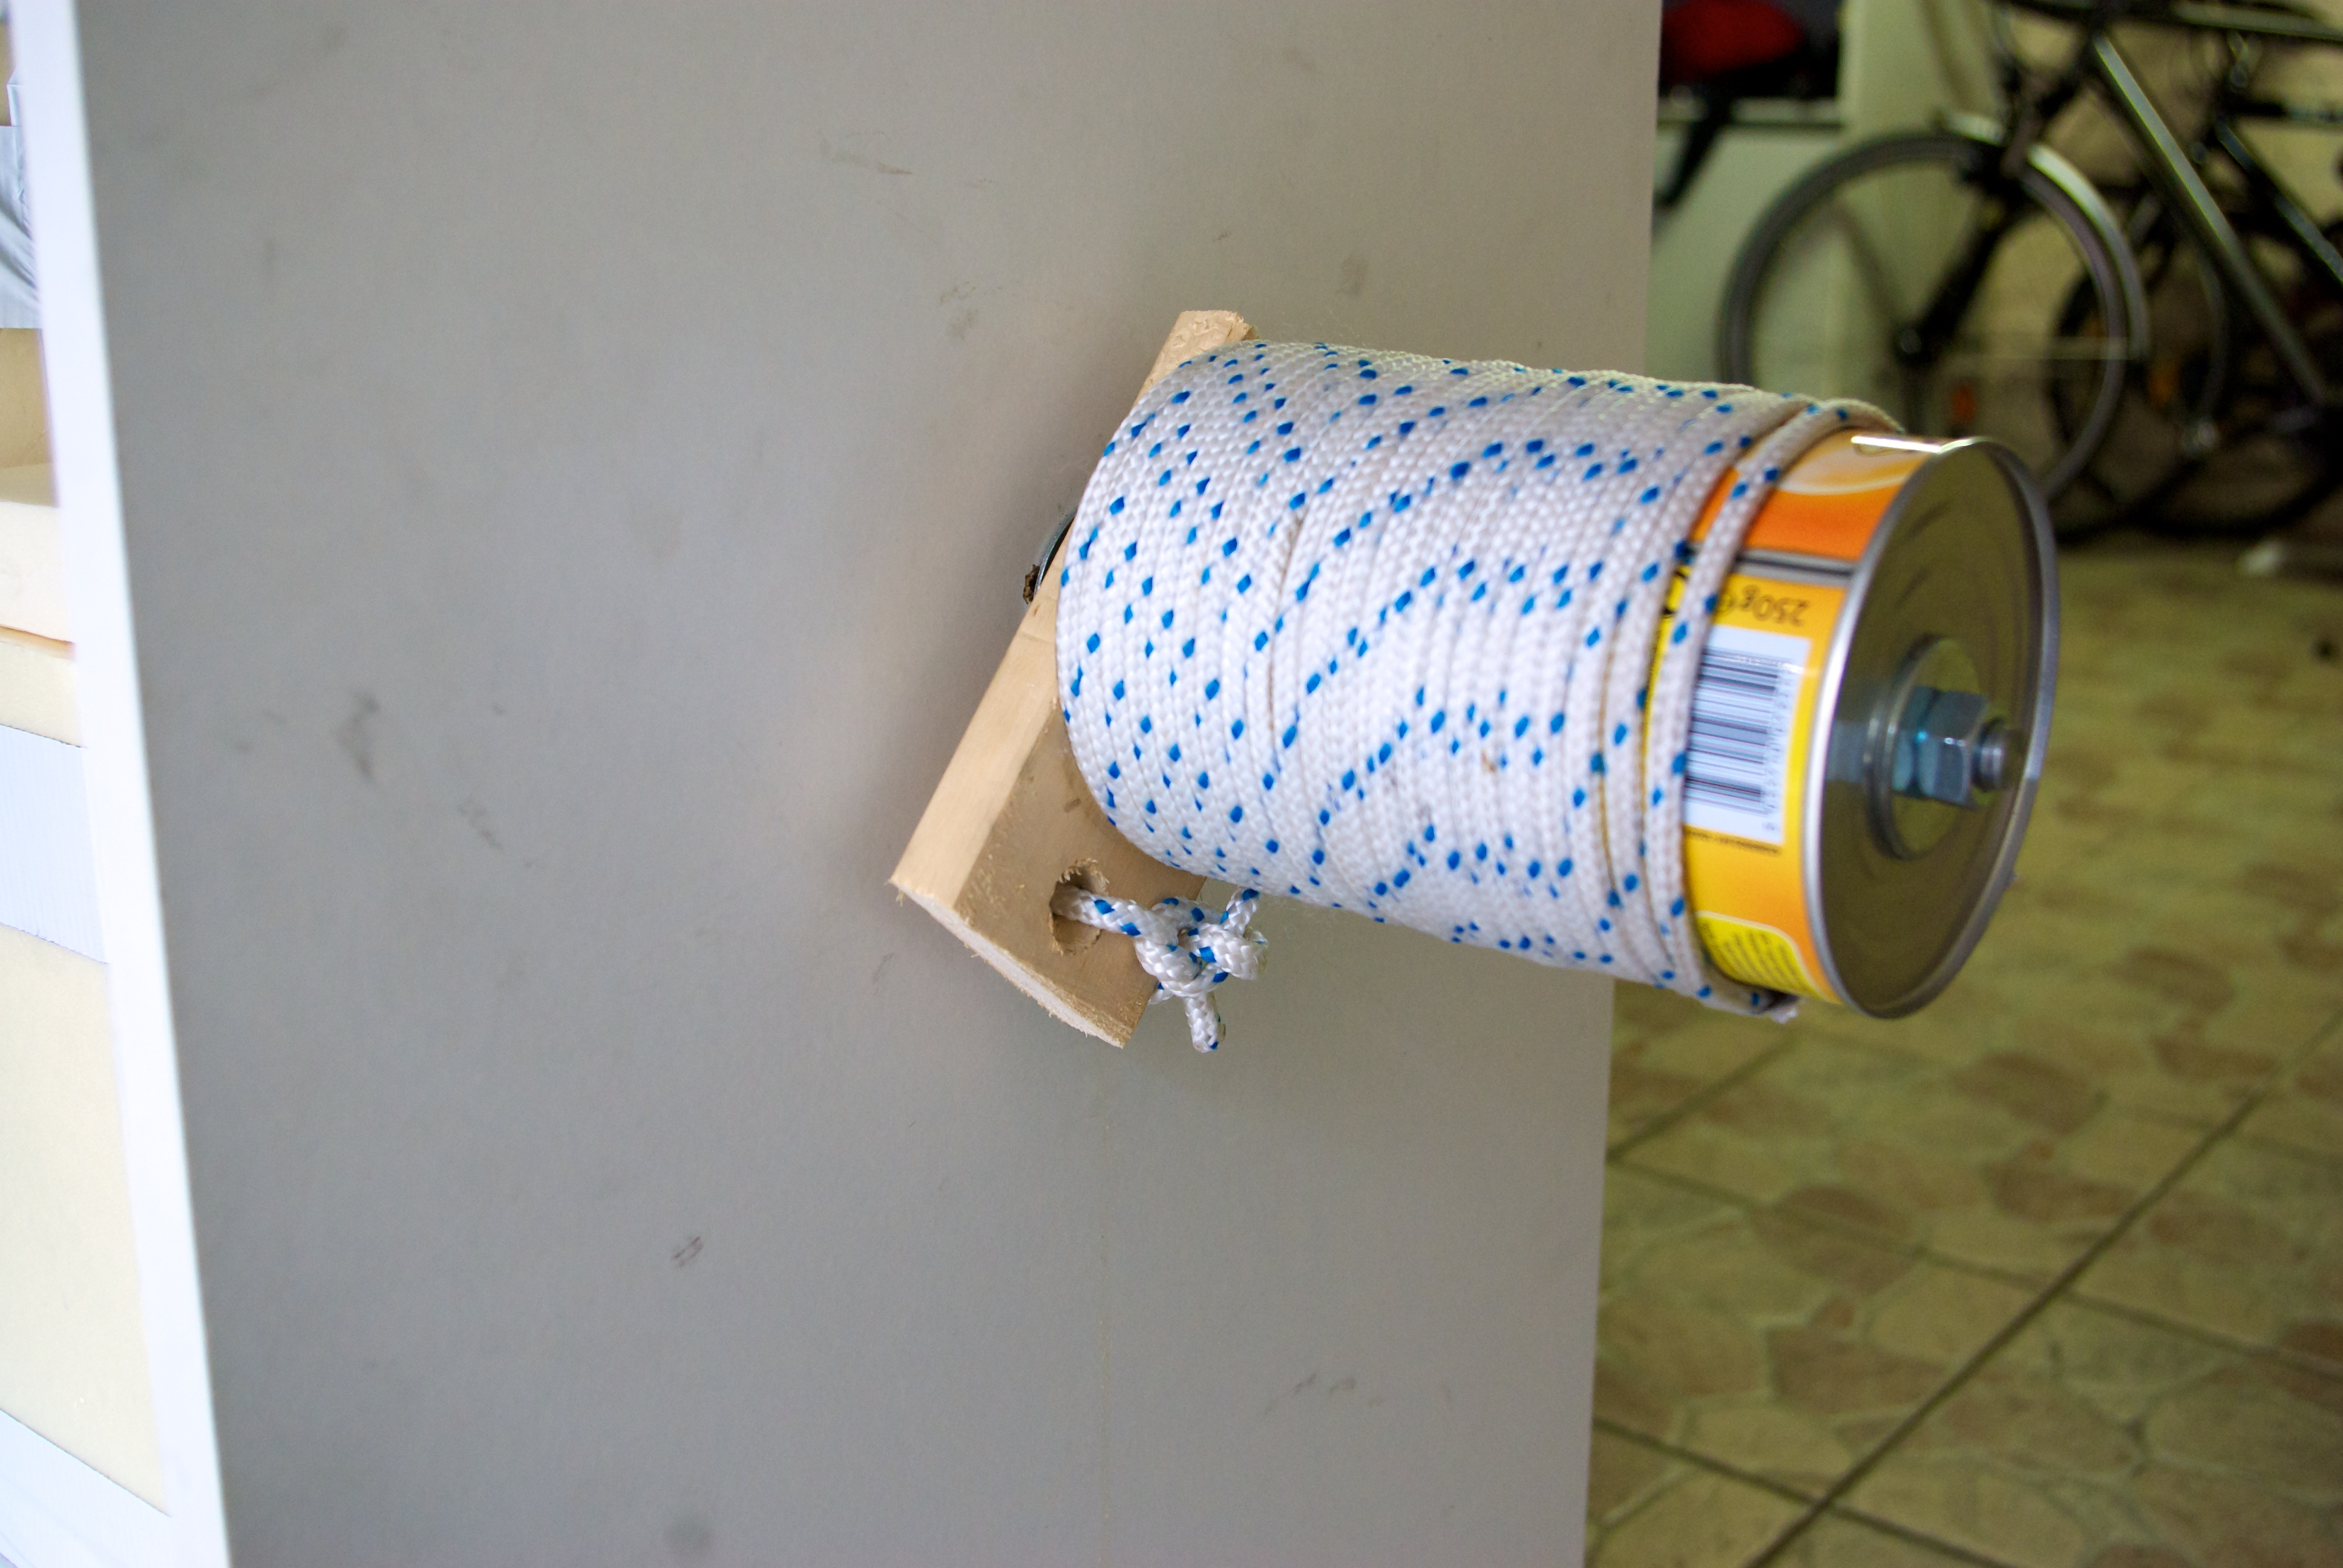
\includegraphics[height=6cm]{photos/appmesure.jpg}
		\caption{\small \label{fig:enrouleur}Enrouleur}
	\end{minipage} \hfill
	\begin{minipage}[t]{6cm}
		\centering
		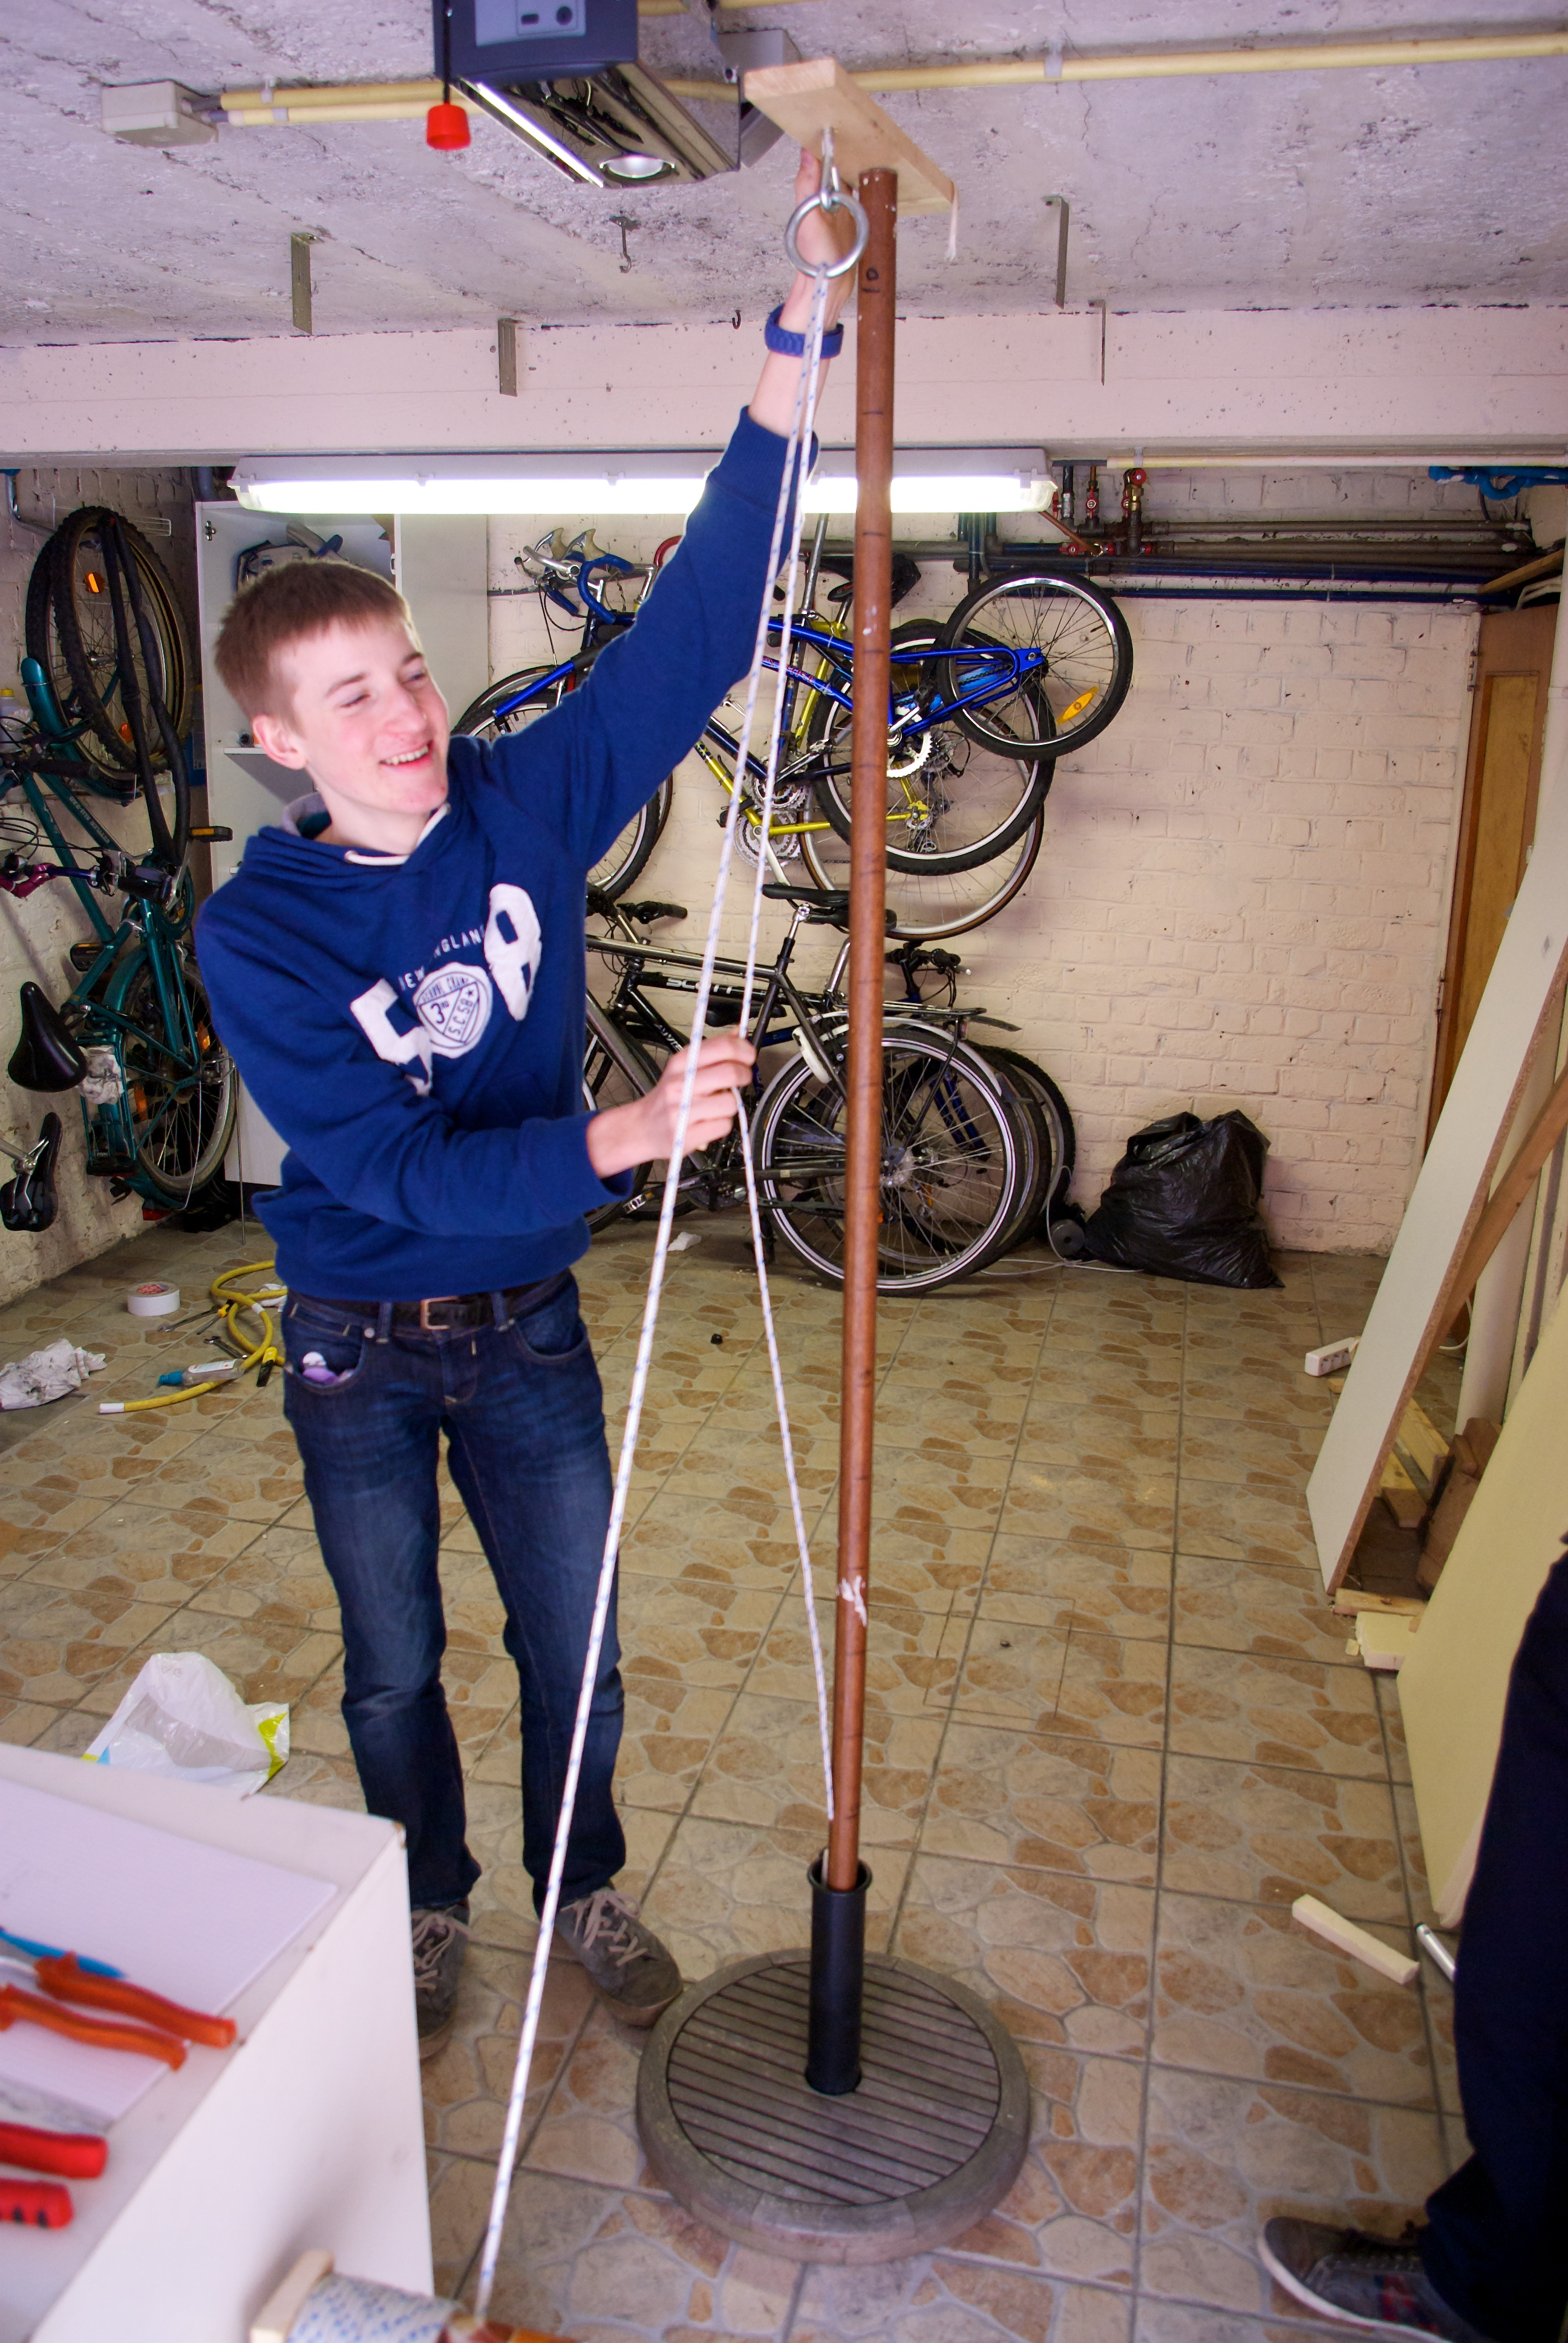
\includegraphics[height=6cm]{photos/appmesure2.jpg}
		\caption{\small \label{fig:appmesure}Appareil de mesure}
	\end{minipage}
\end{figure}




\subsubsection{Exp�rience}
Ainsi, en connaissant la longueur de la chute du poids et en mesurant le temps de chute, il est possible de mesurer sa vitesse. Ensuite, en r�p�tant l'exp�rience plusieurs fois avec des masses diff�rentes, on obtient facilement une grande plage de valeurs afin d'avoir une valeur plus pr�cise du lambda exp�rimental.


\subsubsection{Calcul du lambda exp�rimental}
En consid�rant qu'il n'y a pas de pertes entre le poids et le disque (l'axe du conducteur �tant soutenu par des roulements � bille), on peut consid�rer que la puissance d�velopp�e par le poids est �gale � celle du frein magn�tique. La puissance du frein devient donc~:
\begin{equation*}
P_{frein} = m_{poids}.g.v_{poids}.
\end{equation*}
Pour obtenir le lambda il ne reste donc qu'� diviser ce r�sultat par le carr� de la vitesse du bord du disque. Pour trouver cette vitesse, il est d'abord indispensable de trouver la vitesse angulaire de l'axe. Celle-ci est �gale � la vitesse du poids divis�e par le rayon de l'enrouleur~:
\begin{equation*}
\omega_{3} = \frac{v_{poids}}{r_{enrouleur}}.
\end{equation*}
Pour finalement trouver la vitesse du bord du disque de cuivre, il suffit alors de multiplier cette vitesse angulaire par le rayon du disque~:
\begin{equation*}
v_{disque} = \omega_{3} \, r_{3}'.
\end{equation*}
En divisant finalement la puissance d�velopp�e par le poids par le carr� de la vitesse du bord du disque de cuivre, le $\lambda_{exp�rimental}$ vaut~:
\begin{equation*}
\lambda_{exp�rimental} = \frac{P_{poids}}{v_{3}'^2}
= \frac{m_{poids}.g.v_{poids}}{(\frac{v_{poids}}{r_{enrouleur}} . r_{3}')^2}.
\end{equation*}
Ceci dit, le  $ \lambda_{exp�rimental}$ n'est rien d'autre que la pente du graphe de la puissance en fonction de la vitesse au carr�. En portant les diff�rentes mesures effectu�es et en tra�ant la courbe de tendance des points, on obtient un $ \lambda_{exp�rimental}= \num{52,5}$. 

\begin{figure}[H] %on ouvre l'environnement figure
	\centering
	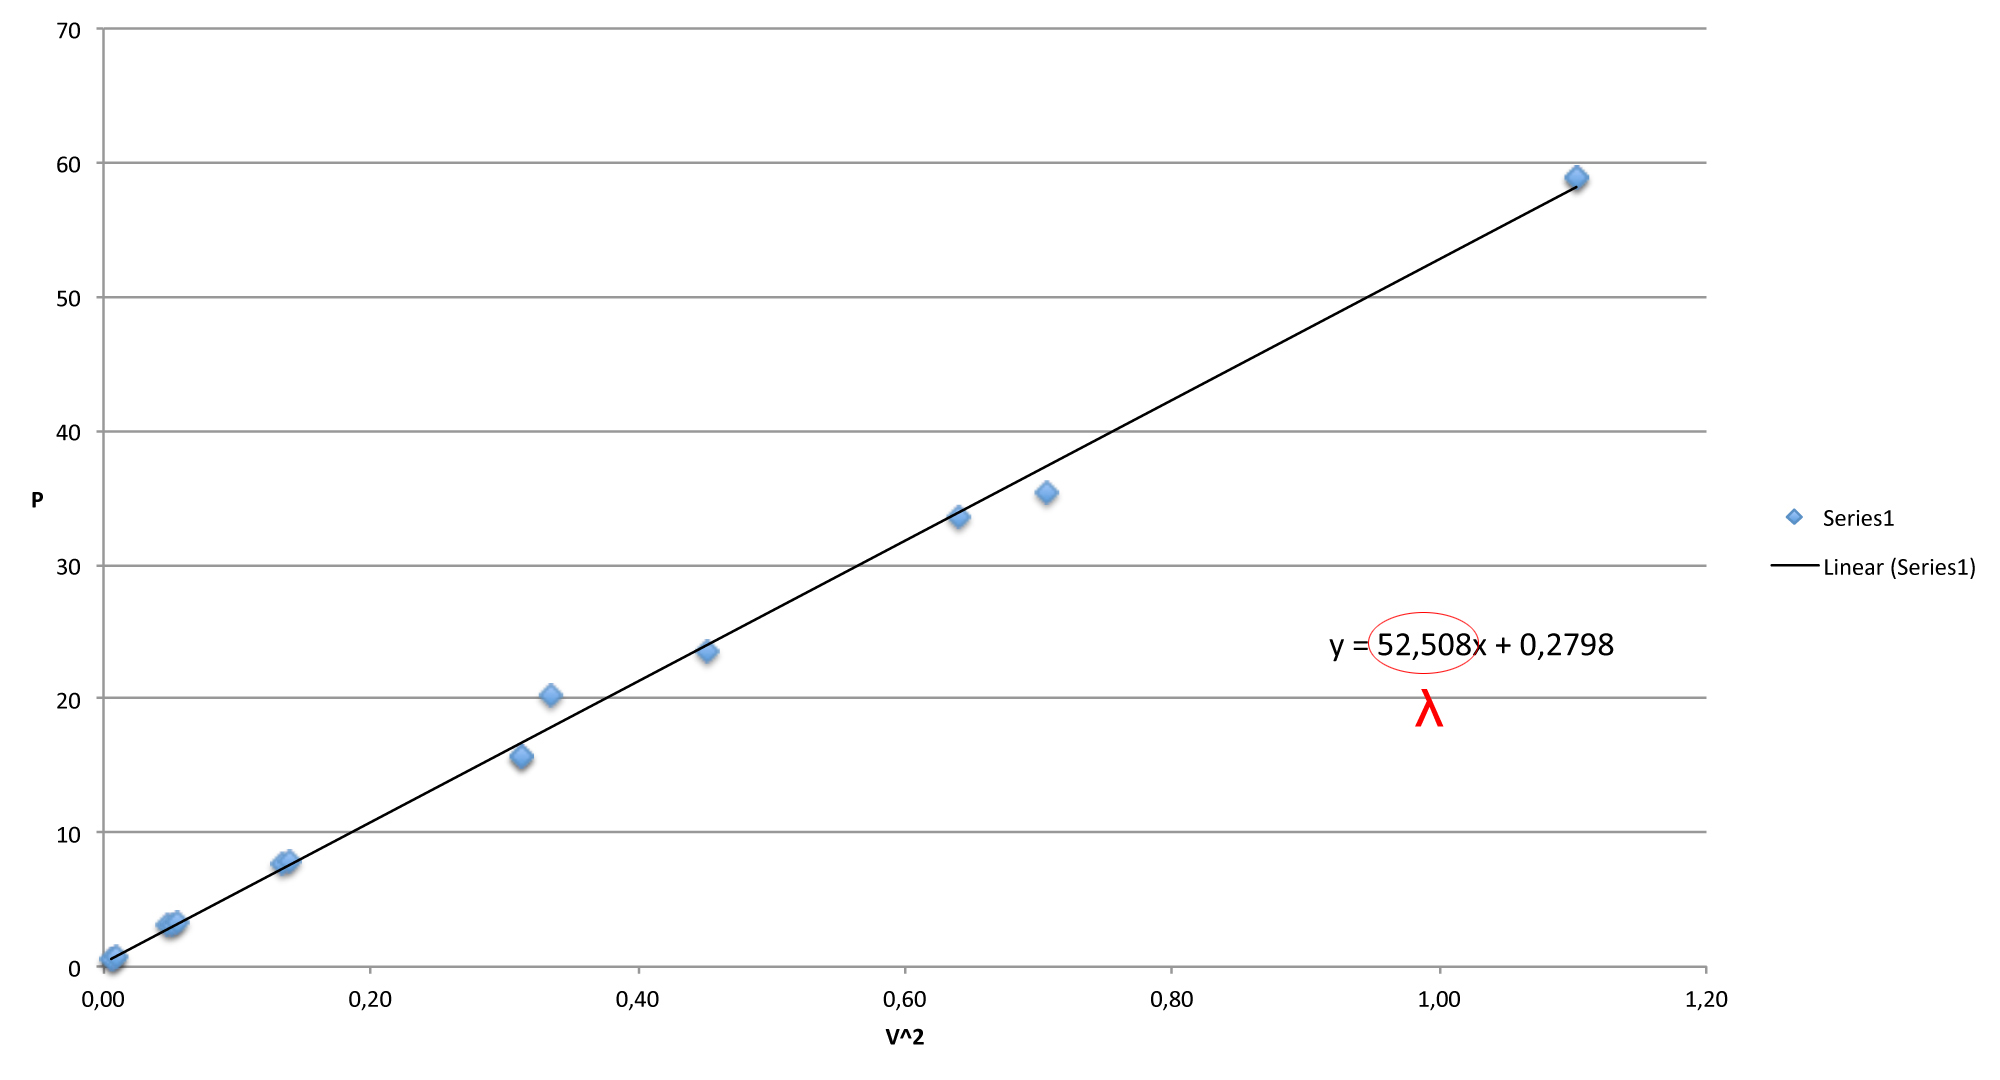
\includegraphics[width=16cm]{graphes/lambda.jpg} %ou image.png, .jpeg etc.
	\caption{\small Graphe de la puissance en fonction de la vitesse au carr�} %la l�gende
	\label{fig:lambda} %l'�tiquette pour faire r�f�rence � cette image
\end{figure} %on ferme l'environnement figure

Ce r�sultat est relativement proche de celui obtenu th�oriquement~: ($\lambda_{th�orique} = \num{34,7}$). La diff�rence s'explique par les pertes dues aux frottements et par les impr�cisions de mod�lisation du champ magn�tique.
%!TEX encoding = IsoLatin
%!TEX root = ./rapport.tex
\subsection{Pertes}

Maintenant que la valeur exp�rimentale de la force de freinage est �tablie, il reste � caract�riser les pertes de l'ergom�tre ainsi qu'� calculer son rendement.

Tout d'abord, les pertes possibles doivent �tre identifi�es puis le(s) rendement(s) de notre ergom�tre doivent �tre mesur�s.
Il y a deux cat�gories de pertes, les pertes thermiques et les pertes m�caniques.
Comme pertes m�caniques, trois principales�ont �t� identifi�es~:
\begin{itemize}
\item frottement de l'axe sur le bord de la cuve,
\item frottement dans la cha�ne,
\item frottement dans les m�canismes du v�lo.
\end{itemize}
Heureusement, � part la premi�re, toutes celles-ci sont mesurables gr�ce � l'appareil de mesure d�crit � la section~\ref{sec:mesure}, bien que les pertes doivent �tre soustraites dans l'appareil de mesure lui-m�me (le frottement de l'axe sur le bord de la cuve �tant pr�sent lors des mesures, il ne peut pas �tre pris en compte) et ajouter les forces de frottement n'apparaissant dans le v�lo que lorsque la structure est sous tension.

Deuxi�mement, les pertes thermiques ont �t� analys�es. Les principales pertes se font par~:
\begin{itemize}
\item les parois de la cuve,
\item le disque/conducteur (puis via l'axe)
\item �change avec l'air ambiant via les ouvertures du haut du caisson
\end{itemize}
Afin de mesurer ces pertes, la cuve a �t� remplie d'eau chaude � 42�C,  puis elle a �t� plac�e dans l'ergom�tre et la diminution de la temp�rature de l'eau a �t� mesur�e. La conclusion de cette exp�rience fut que, si la temp�rature de l'eau est 25�C plus haute que la temp�rature ext�rieure, au plus 1�C par quart d'heure est perdu.


\subsection{Rendement}
Le rendement est d�fini comme �tant la puissance utile divis�e par la puissance totale $\eta_{tot}=\frac{P_{utile}}{P}$. Ici, il est �gal � $\eta_{m�ca} . \eta_{therm}$.
\subsubsection{Rendement m�canique}

Le rendement m�canique ($\eta_{m�ca}$) est �gal � $\frac{P_{j}}{P_{j}+P_{f}}$,
$P_{j}$ �tant la puissance de chauffe des aimants et $P_{f}$ la puissance des frottements.
On peut donc assimiler $P_{j}$ � $\lambda_{exp�rimental}.v_{3}'^2$ (en n�gligeant donc les frottements dans les roulements de la cuve)
et $P_{f}$ � $\lambda  ^{\prime}.v_{3}^2$. $\lambda  ^{\prime}$ �tant le coefficient liant la puissance des pertes au carr� de la vitesse du disque et �tant mesur� de la m�me fa�on de $\lambda_{exp}$ mais en retirant le frein magn�tique. Le coefficient $\lambda  ^{\prime}$ valant \num{6,5}.
\begin{equation*}
\eta_{m�ca} = \frac{P_{j}}{P_{j}+P_{f}} = \frac{\lambda_{exp} v_{3}'^2}{\lambda_{exp} v_{3}'^2+\lambda  ^{\prime}.v_{3}'^2} = \frac{\lambda_{exp}}{\lambda_{exp}+\lambda  ^{\prime}}
\end{equation*}
Par cons�quent l'ergom�tre a un rendement m�canique de $\frac{52,5}{52,5+6,5}= 0,88$.

\subsubsection{Rendement thermique}

Le rendement thermique ($\eta_{therm}$) est �gal �~:
\begin{equation*}
1-\frac{H}{P_{j}},
\end{equation*}
$H$ �tant la puissance des pertes thermiques, car~:
\begin{equation*}
\eta_{therm} = \frac{P_{u}}{P_{u}+H} = \frac{P_{u}}{P_{j}} = \frac{P_{j}-H}{P_{j}}= 1-\frac{H}{P_{j}},
\end{equation*}
avec $P_{u}$ �tant la puissance r�ellement utile pour chauffer l'eau.
Etant donn� que les pertes thermiques d�pendent de la diff�rence de temp�rature entre l'eau et l'ext�rieur, on peut consid�rer que si l'exp�rience commence � temp�rature ambiante et que l'eau n'est pas chauff�e trop longtemps, les pertes seront nulles et donc le rendement �gal � 100 \%.

Cependant, afin de voir ce que vaudrait le rendement thermique apr�s plusieurs heures de chauffe, l'eau a �t� port�e � 42�C pour mesurer la diminution de temp�rature avec le temps (la temp�rature ambiante valant 12�C). A cette temp�rature, les pertes sont de l'ordre de 50W, soit un rendement thermique d'environ 82\%.

\subsubsection{Conclusion}

Rappelons-nous du rendement total, qui d�pend de $\eta_{m�ca}$ et $\eta_{therm}$. Tant que la temp�rature ambiante est proche de celle de l'eau, le rendement thermique est proche de 100\%, et $\eta_{total}\simeq88\%$.

Au fur et � mesure que l'eau chauffe, le rendement thermique diminue, de m�me que le rendement total. Lorsque la diff�rence de temp�rature entre l'eau et le milieu ext�rieur atteint une trentaine de degr�s, $\eta_{total}\simeq72\%$.
\newpage
%!TEX encoding = IsoLatin
%!TEX root = ./rapport.tex
\newpage
\section{Fonctionnement de groupe}

Le groupe �tait initialement compos� de 6 personnes dirig�es par un chef d'�quipe. Un membre du groupe ayant arr�t� les �tudes d'ing�nieur civil, le groupe ne comptait plus que 5 personne � partir du mois de f�vrier.

Chaque semaine, au moins une r�union a lieu. Tous les membres du groupe ainsi que le chef de projet sont pr�sents.
A ces r�unions, un secr�taire est d�sign�. Ce secr�taire a pour t�che de remettre, apr�s la r�union, un rapport de la r�union sur dropbox. Ainsi, tous les membres du groupe peuvent se rafra�chir la m�moire avant la r�union suivante.

Ces rapports sont �galement pratiques quand une personne n'a pas pu �tre pr�sente � une r�union. Elle peut alors lire ce qui a �t� dit � la r�union � laquelle elle n'�tait pas pr�sente et �tre au courant de l'avancement du projet.
Pendant ces r�unions, chaque membre du groupe rapporte le travail et les avancements qu'il a effectu�s pour le projet durant cette semaine. De cette fa�on, le chef d'�quipe et les membres du groupe sont au courant de l'�tat d'avancement du projet.

C'est aussi au cours de ces r�unions que les d�cisions importantes sont prises. Le groupe parle notamment de la d�cision � prendre avec le chef de projet qui donne son avis pour que le groupe puisse prendre la d�cision la plus avantageuse.
A la fin de chaque r�union, les t�ches � effectuer pour la prochaine r�union sont r�parties �quitablement entre les membres du groupe. 

Presque chaque semaine, le groupe fixe une deuxi�me r�union sans la pr�sence du chef de projet. 
C'est notamment durant ces r�unions que le travail sur l'ergom�tre est effectu�. Le groupe discute �galement de l'avancement des t�ches de chacun et, si un membre du groupe ne comprend pas quelque chose, les autres membres du groupe lui fournissent des explications. 

En dehors des r�unions, le groupe communique essentiellement par mail. Les \bsc{SMS} sont aussi utilis�s, ainsi que Skype qui a �t� un moyen d'organiser des vid�oconf�rences, permettant de se retrouver (ne serait-ce que virtuellement) facilement et rapidement.

Le groupe n'a pas toujours �t� tr�s ponctuel durant le premier quadrimestre, mais s'est n�anmoins bien am�lior� au deuxi�me quadrimestre. Toutes les t�ches ont �t� effectu�es � temps, contrairement � ce qu'il arrivait parfois au premier quadrimestre, ralentissant  l'avancement du projet. Le groupe n'a donc plus pris de retard sur le planning et tout s'est mieux d�roul�.

L'ambiance au sein du groupe est rest�e bonne et le travail a toujours �t� partag� de fa�on �quitable entre les membres du groupe.

%\subsection{Gestion du groupe par le chef d'�quipe}
%
%Le chef de groupe conseille et aide les membres concernant leur travail. Il s'assure de la bonne compr�hension du projet par les membres et demande r�guli�rement des mises � jours sur l'avancement des diff�rentes t�ches � effectuer. Il n'est pas rare que le chef de projet demande en r�union des comptes rendus des activit�s du groupe, pour voir si les d�lais sont respect�s et si le groupe ne s'oriente pas vers une mauvaise piste.
%
%Le contact entre celui-ci et le reste du groupe en dehors des r�unions s'effectue par mails et par sms, afin de permettre une bonne communication entre tous les membres. Le chef de groupe intervient notamment dans les choix cruciaux, s'assurant du bien-fond� des d�cisions, mais aussi dans la r�partition du travail pour que cette charge soit �quitablement distribu�e entre chaque membre.
\newpage
%!TEX encoding = IsoLatin
%!TEX root = ./rapport.tex
\newpage
\section{Conclusion}

Le projet tire � sa fin. L'ergom�tre a �t� construit avec succ�s et il est donc temps pour le groupe d'�crire tout ce qu'il a appris durant ce travail. Ce projet nous a enrichi dans bien des domaines dont quelque-uns sont d�velopp�s dans cette conclusion.

La premi�re chose que ce travail nous a appris, c'est � faire des recherches sur des sujets scientifiques dont on n'a au pr�alable aucune notion. Chercher des livres dans une biblioth�que scientifique, trouver des sources fiables sur internet, etc. 

Ce travail nous a �galement appris que l'�criture d'un rapport scientifique n'est pas une chose qui s'improvise. Elle se fait notamment en parall�le avec le d�roulement du projet.
Ce projet nous a �galement donn� de la joie, particuli�rement de savoir que notre ergom�tre fonctionnait presque parfaitement, apr�s avoir r�ussi � r�soudre tous les probl�mes. 

Tout au long du parcours, nous avons �galement appris que certaines parties d'un projet �taient moins amusantes que d'autres, mais qu'elles ne devaient en aucun cas �tre n�glig�es. Ces t�ches moins dr�les sont notamment aussi indispensables au bon d�roulement d'un projet que les parties agr�ables. 

Tous ces �l�ments et bien d'autres encore ont donc permis � ce groupe d'�voluer, tant du c�t� humain que du c�t� technique de la gestion d'un projet.

%\input{chap1}
%\input{chap2}
%\input{chap3}

%%%%%%%%%%%%%%%
%Annexes
%%%%%%%%%%%%%%%
\newpage
\pagenumbering{Roman}
\appendix
%!TEX encoding = IsoLatin
%!TEX root = ./rapport.tex
\section{Annexes}

\subsection{Budget}

\begin{table}[htdp]
\begin{center}
\begin{tabular}{|l|l|}
\hline Libell� & Prix\\
\hline \hline Aimants & \EUR{24.80}\\
\hline Plaque de cuivre & \EUR{23.20}\\
\hline Isolant & \EUR{12.05}\\
\hline Corde & \EUR{3.67} \\
\hline Poulie & \EUR{3.05} \\
\hline Porte-v�lo & \EUR{50} \\
\hline \hline Total & \EUR{116,67} \\
\hline
\end{tabular}
\end{center}
\end{table} 

%\subsection{Mesure du champ d'un aimant}
%
%Soit $w_{m}$ la densit� de l'�nergie m�canique.
%
%$$w_{m}=\frac{1}{2\mu_{0}}B^{2}$$
%O� $\mu_{0}=4\pi 10^{-7}$ est la perm�abilit� magn�tique du vide.\\
%$w_{M}$ est l'�nergie m�canique et est donc d�finie par :
%
%$$w_{M}=w_{m}V=\frac{1}{2\mu_{0}}B^{2}V$$
%O� $V$ est le volume de l'entre-fer.\\
%Quand deux aimants sont coll�s l'un � l'autre, $V=0$, donc $w_{M}=0$
%
%\begin{figure}[H] %on ouvre l'environnement figure
%	\centering
%	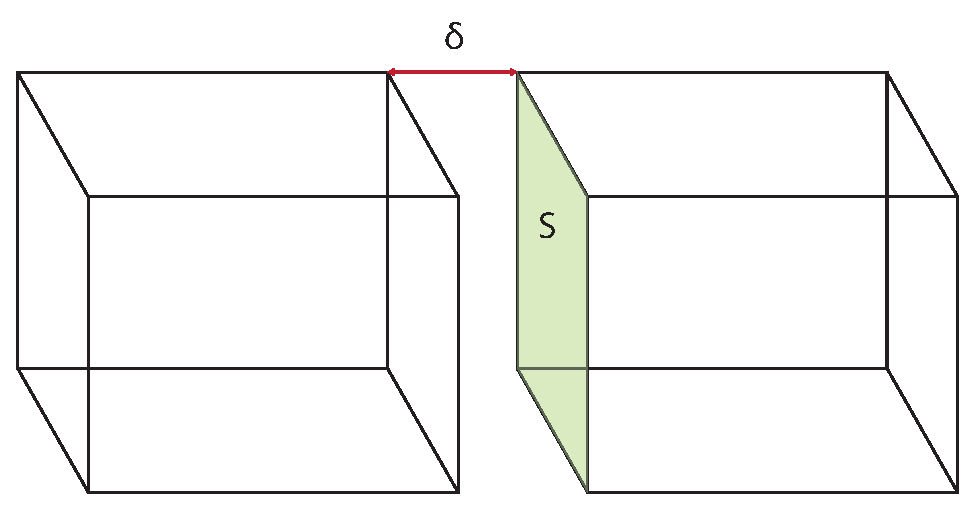
\includegraphics[width=10cm]{schema6.eps} %ou image.png, .jpeg etc.
%	\caption{\small Entre-fer des aimants.} %la l�gende
%	\label{aimants} %l'�tiquette pour faire r�f�rence � cette image
%\end{figure} %on ferme l'environnement figure
%
%Quand ces deux aimants sont espac�s d'une longueur $\delta$, (Figure~\ref{aimants})
%
%$$w_{M}=\frac{1}{2\mu_{0}}B^{2}S\delta$$
%
%O� S est la surface de l'entre-fer. ($V=S\delta$)
%
%Or, l'�nergie m�canique est aussi (travail) : $w_{M}=F_{M}\delta$
%
%Donc : $$F_{M}=\frac{1}{2\mu_{0}}B^{2}S$$
%
%Il suffit ensuite d'isoler $B$ en fonction de la force exerc�e sur un des aimants pour les s�parer :
%
%$$B=\sqrt{\frac{2F_{M}\mu_{0}}{S}}$$

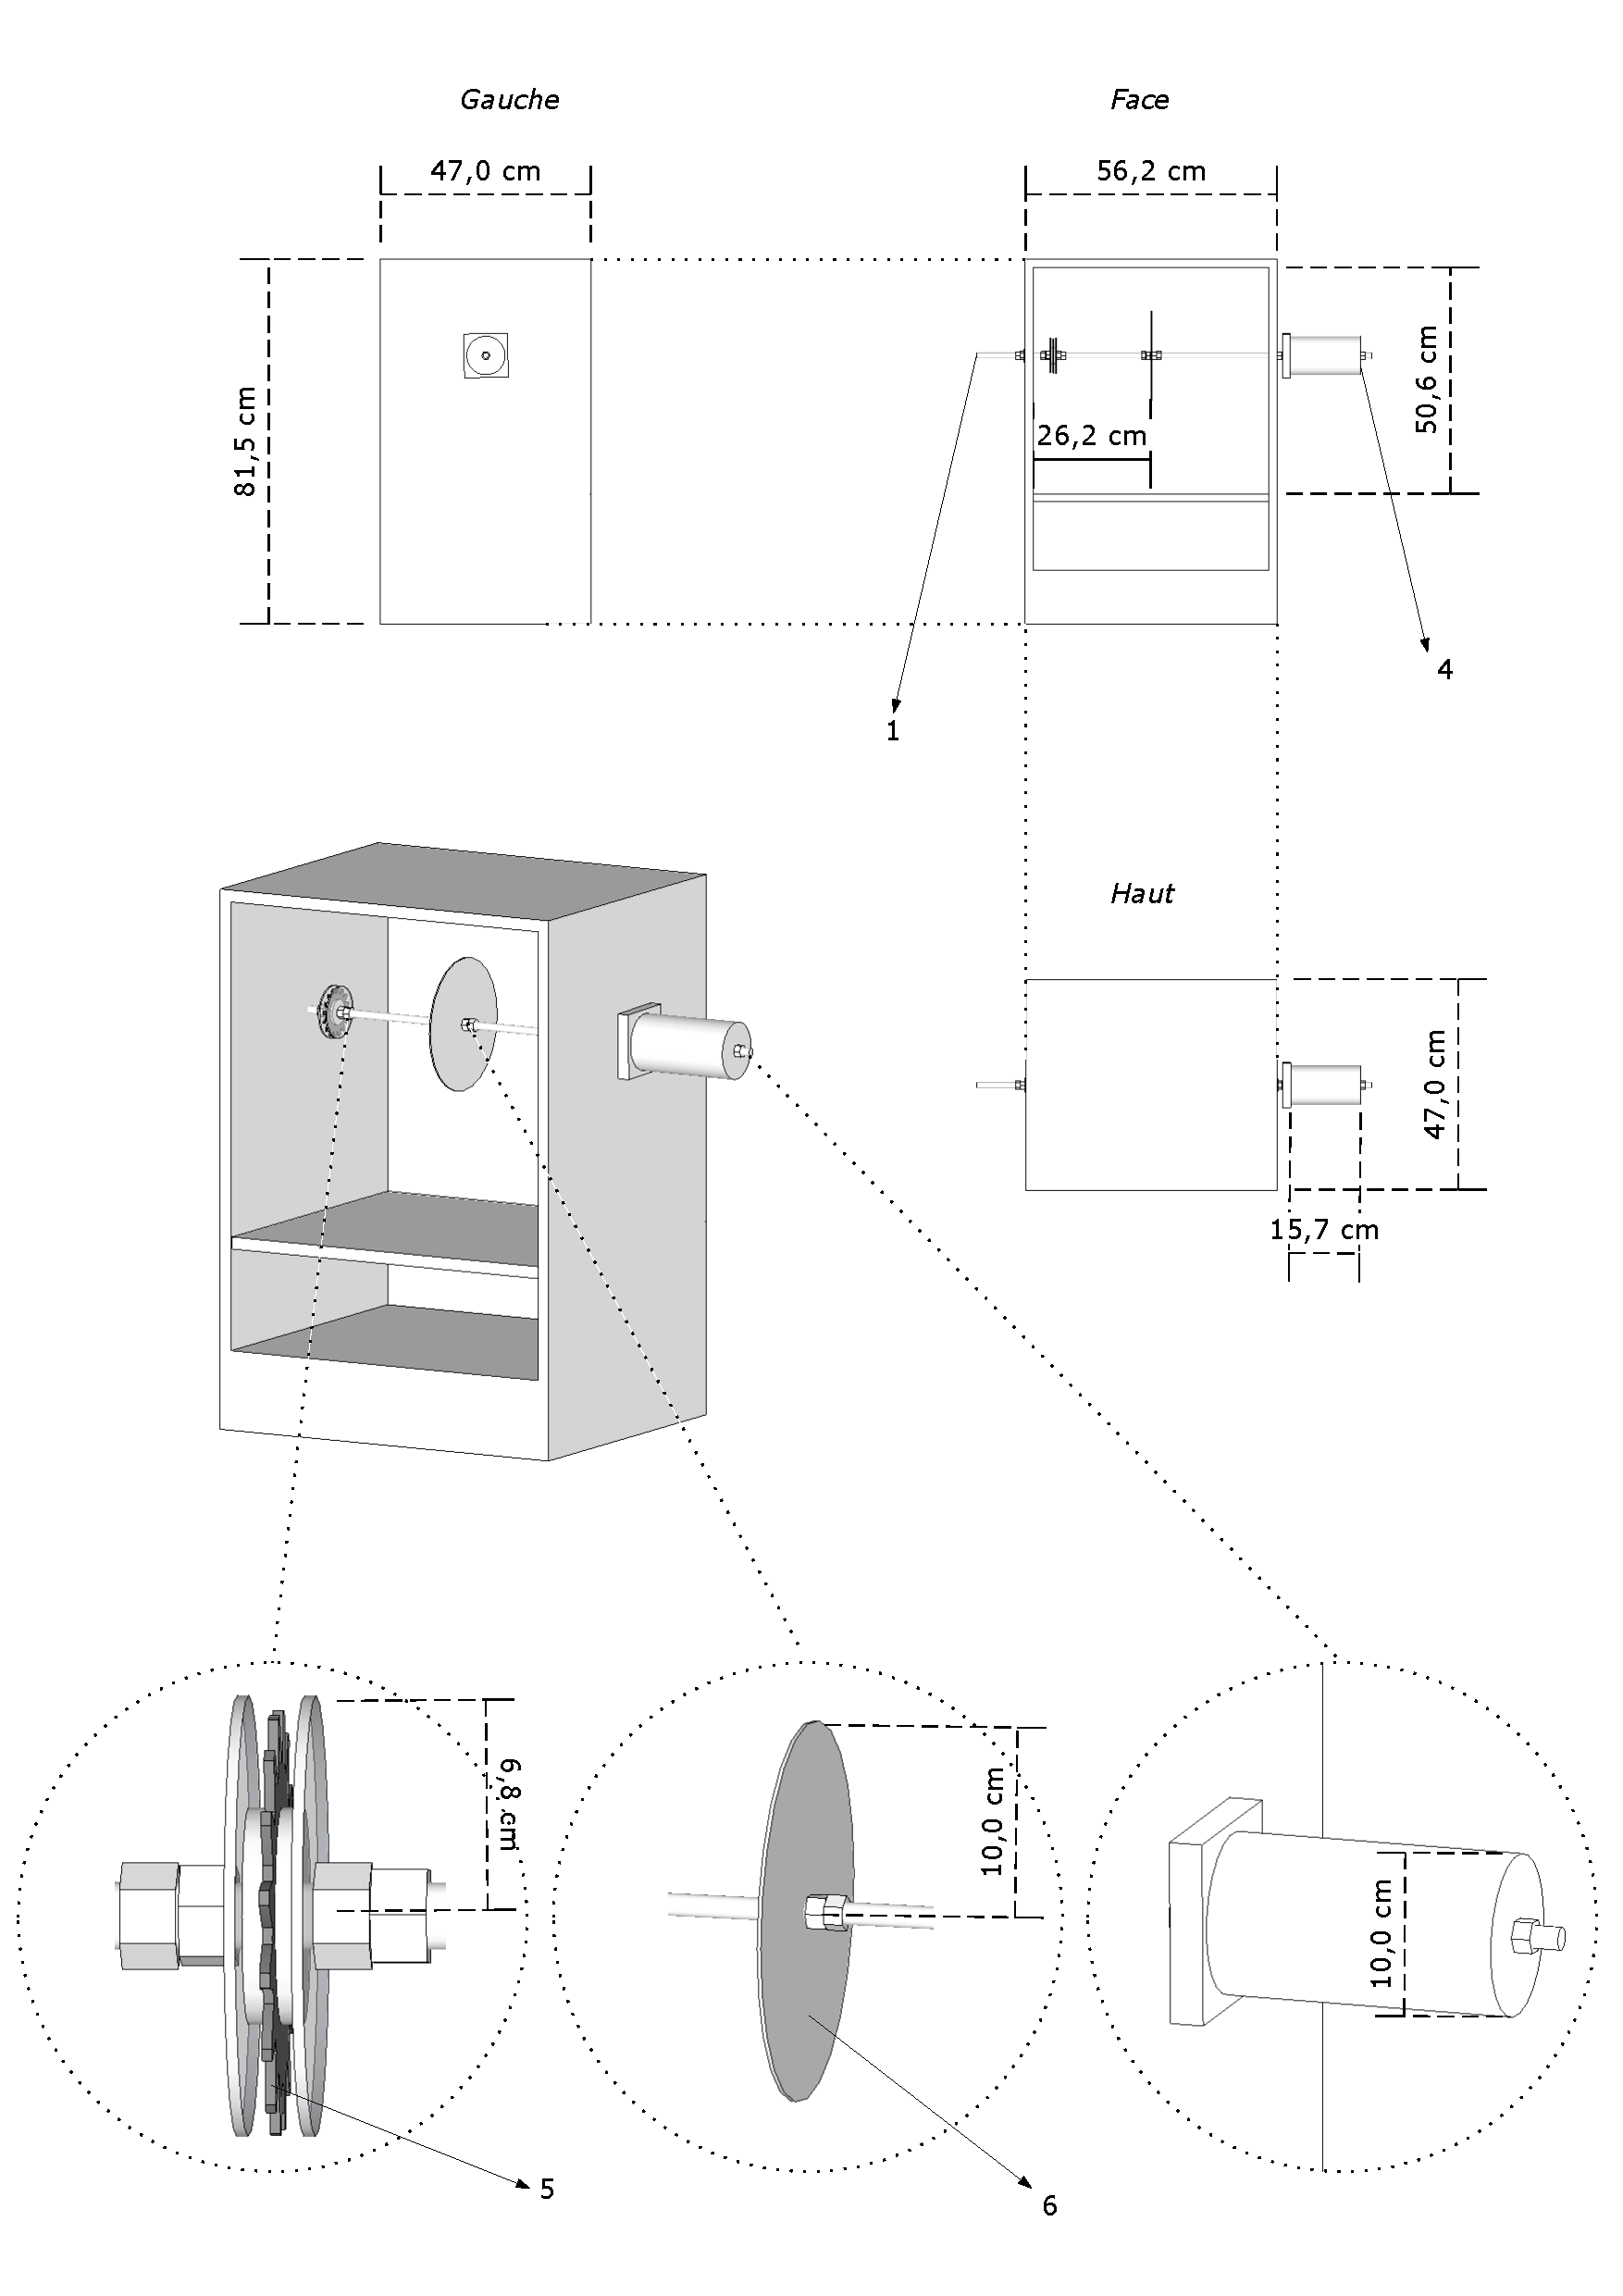
\includepdf{plan1.pdf}
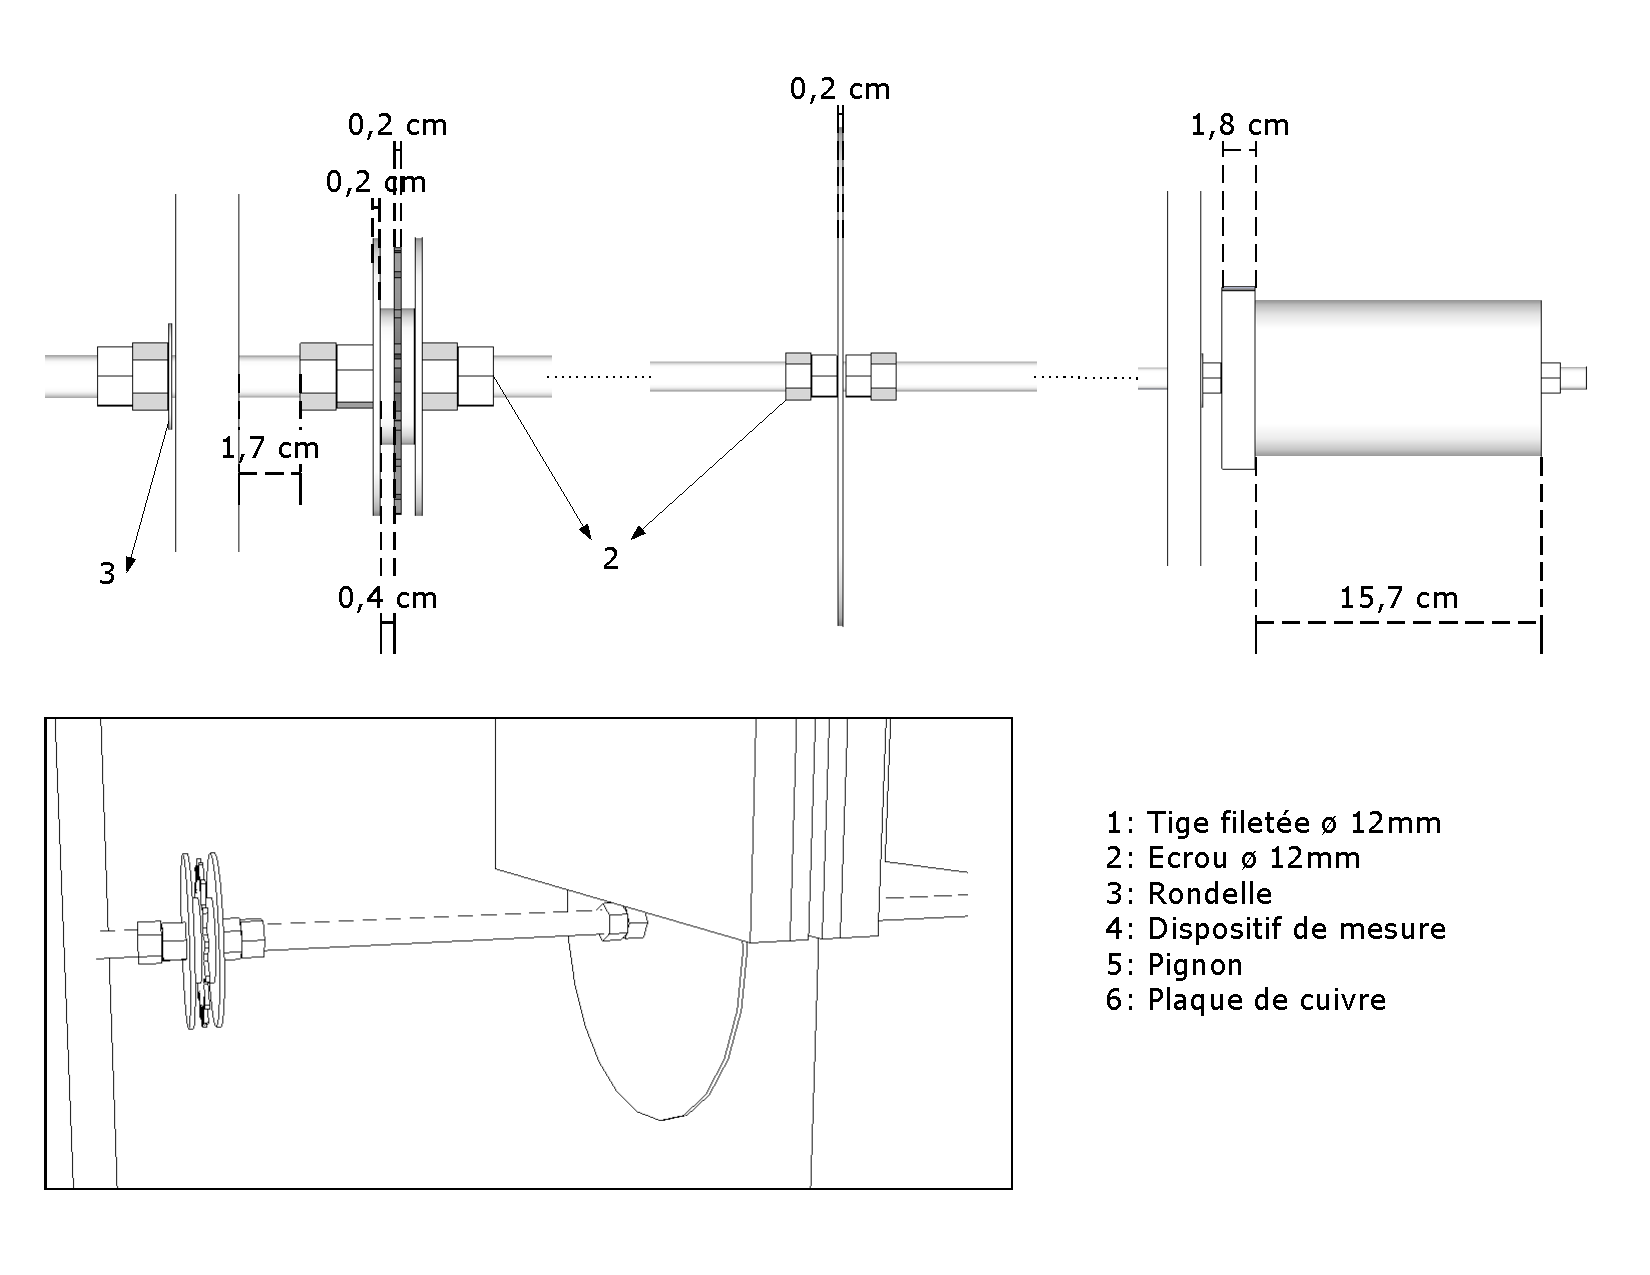
\includepdf[fitpaper]{plan2.pdf}

%\subsection{Photos}

%\begin{figure}[H] %on ouvre l'environnement figure
%	\centering
%	\includegraphics[width=10cm]{roulement.eps} %ou image.png, .jpeg etc.
%	\caption{\small R�cup�ration de roulements � bille pour soutenir l'axe} %la l�gende
%	\label{roule} %l'�tiquette pour faire r�f�rence � cette image
%\end{figure} %on ferme l'environnement figure

 

%%%%%%%%%%%%%%%
%Fin
%%%%%%%%%%%%%%%
%!TEX encoding = IsoLatin
%!TEX root = ./rapport.tex

% ******************
% * fichier de fin *
% ******************
\newpage
%\listoftables
%\listoffigures
\bibliographystyle{plain}
\bibliography{bibliographie}

\end{document}

